% $Header: /home/vedranm/bitbucket/beamer/solutions/generic-talks/generic-ornate-15min-45min.en.tex,v 90e850259b8b 2007/01/28 20:48:30 tantau $

\documentclass{beamer}

% This file is a solution template for:

% - Giving a talk on some subject.
% - The talk is between 15min and 45min long.
% - Style is ornate.



% Copyright 2004 by Till Tantau <tantau@users.sourceforge.net>.
%
% In principle, this file can be redistributed and/or modified under
% the terms of the GNU Public License, version 2.
%
% However, this file is supposed to be a template to be modified
% for your own needs. For this reason, if you use this file as a
% template and not specifically distribute it as part of a another
% package/program, I grant the extra permission to freely copy and
% modify this file as you see fit and even to delete this copyright
% notice. 


\mode<presentation>
{
  \usetheme{Warsaw}
  % or ...

  \setbeamercovered{transparent}
  % or whatever (possibly just delete it)
}


\usepackage[english]{babel}
% or whatever

\usepackage[latin1]{inputenc}
% or whatever

\usepackage{times}
\usepackage[T1]{fontenc}
% Or whatever. Note that the encoding and the font should match. If T1
% does not look nice, try deleting the line with the fontenc.


\usepackage{marvosym} % For \Smiley
\usepackage{verbatim} % for \verbatiminput

\title[Limited Information Strategies for Topological Games] % (optional, use only with long paper titles)
{Limited Information Strategies for Topological Games}

\subtitle
{GSC Scholars' Forum / AU Research Week 2013} % (optional)

\author%[Author, Another] % (optional, use only with lots of authors)
{Steven~Clontz}%\inst{1} \and S.~Another\inst{2}}
% - Use the \inst{?} command only if the authors have different
%   affiliation.

\institute[Auburn University] % (optional, but mostly needed)
{
  %\inst{1}%
  Department of Mathematics and Statistics\\
  Auburn University}
  %\and
  %\inst{2}%
  %Department of Theoretical Philosophy\\
  %University of Elsewhere}
% - Use the \inst command only if there are several affiliations.
% - Keep it simple, no one is interested in your street address.

\date[13-02-27] % (optional)
{February 27, 2013}

\subject{Limited Information Strategies for Topological Games}
% This is only inserted into the PDF information catalog. Can be left
% out. 



% If you have a file called "university-logo-filename.xxx", where xxx
% is a graphic format that can be processed by latex or pdflatex,
% resp., then you can add a logo as follows:

 \pgfdeclareimage[height=1cm]{university-logo}{auburn_logo.png}
 \logo{\pgfuseimage{university-logo}}



% Delete this, if you do not want the table of contents to pop up at
% the beginning of each subsection:
%\AtBeginSubsection[]
%{
%  \begin{frame}<beamer>{Outline}
%    \tableofcontents[currentsection,currentsubsection]
%  \end{frame}
%}


% If you wish to uncover everything in a step-wise fashion, uncomment
% the following command: 

%\beamerdefaultoverlayspecification{<+->}

% My game notational definitions

\newcommand{\win}{\uparrow}
\newcommand{\prewin}{\uparrow_{\text{predetermined}}}
\newcommand{\markwin}{\uparrow_{\text{Mark\"ov}}}
\newcommand{\tactwin}{\uparrow_{\text{tactic}}}
\newcommand{\ktactwin}[1]{\uparrow_{#1\text{-tactic}}}
\newcommand{\kmarkwin}[1]{\uparrow_{#1\text{-Mark\"ov}}}
\newcommand{\codewin}{\uparrow_{\text{coding}}}
\newcommand{\limitwin}{\uparrow_{\text{limit}}}
\newcommand{\oneptcomp}[1]{#1^*}
\newcommand{\congame}[2]{Con_{O,P}(#1,#2)}
\newcommand{\clusgame}[2]{Clus_{O,P}(#1,#2)}
\newcommand{\lfkpgame}[1]{LF_{K,P}(#1)}
\newcommand{\lfklgame}[1]{LF_{K,L}(#1)}


\begin{document}

\begin{frame}
  \titlepage

  {\tiny http://www.stevenclontz.com/AURW2013/}
\end{frame}

\begin{frame}{Table of Contents}
  \tableofcontents
  % You might wish to add the option [pausesections]
\end{frame}


% Since this a solution template for a generic talk, very little can
% be said about how it should be structured. However, the talk length
% of between 15min and 45min and the theme suggest that you stick to
% the following rules:  

% - Exactly two or three sections (other than the summary).
% - At *most* three subsections per section.
% - Talk about 30s to 2min per frame. So there should be between about
%   15 and 30 frames, all told.

\section{Introduction}

\subsection{Abstract}

\begin{frame}{Abstract}%{Subtitles are optional.}
  % - A title should summarize the slide in an understandable fashion
  %   for anyone how does not follow everything on the slide itself.

  \begin{itemize}
  \item
    Many definitions of topological properties can be elegantly described in terms of a two-player ``topological game'' of countably infinite length. 
  % \pause
  \item
    In a topological game, a property of the topological space being played upon is characterized by whether one player or another has a ``winning strategy'', a strategy which cannot be countered by any possible play by the opponent. 
  % \pause
  \item 
    The presenter's research involves investigating several topological games from the literature for properties characterized by the existence of winning ``limited information'' strategies.
  \end{itemize}
  \pause
Might want some background first...
\end{frame}

\section{Topology \& Infinite Length Games}

\subsection{Topology}

\begin{frame}{What is Topology?}

  \begin{itemize}
  \item
    Topology is, put simply, the study of mathematical ``spaces''.
  \pause
  \item
    Most of us have learned about the (usual) topology of the real line and the $xy$-plane in calculus.
  \end{itemize}
  \begin{center}
    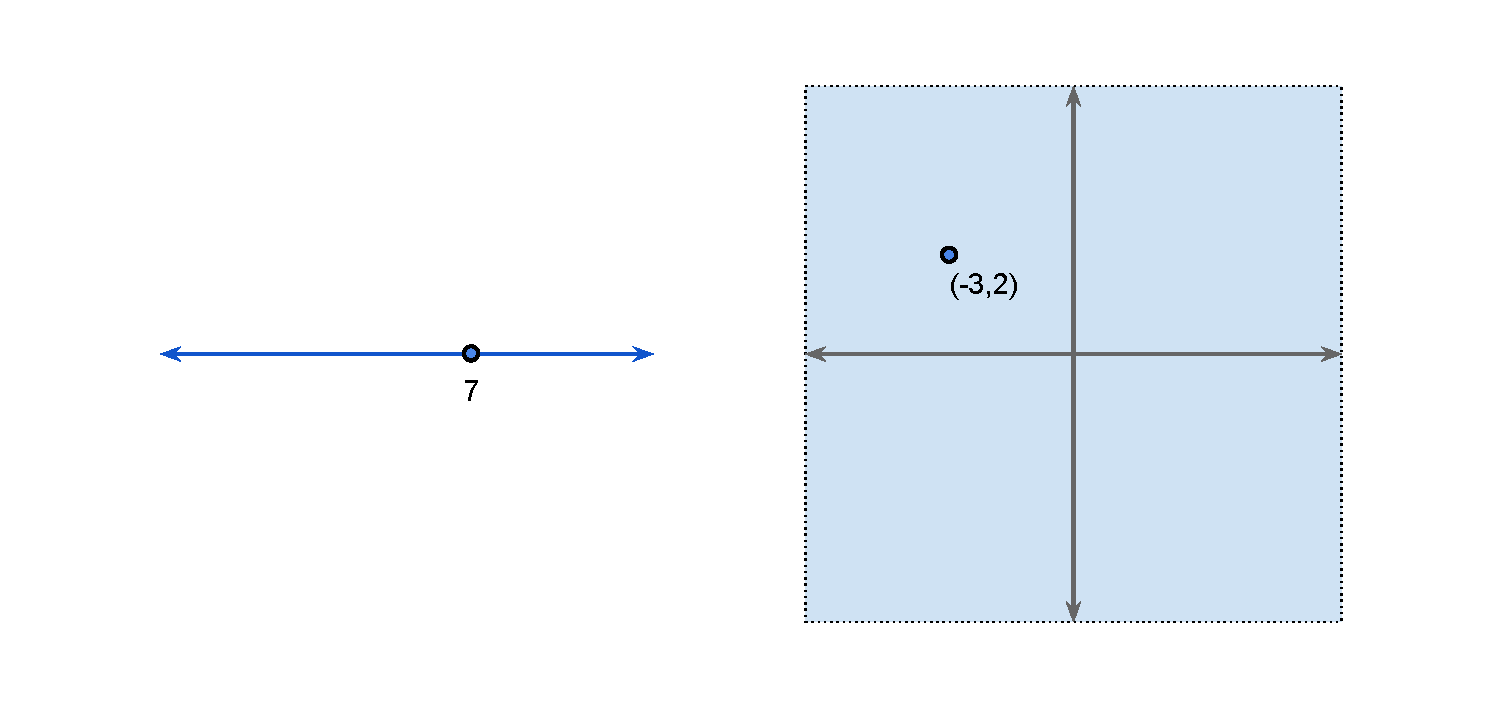
\includegraphics[height=4cm]{images/r_r2}
  \end{center}
\end{frame}
\begin{frame}
  \begin{itemize}
  \item
    Topology is chiefly concerned with the ``structure'' of mathematical spaces.
  \pause
  \item
    A simple example of a topological observation is that removing a point from the real line splits it into two separated pieces, while removing a point from the real plane does not.
  \end{itemize}
  \begin{center}
    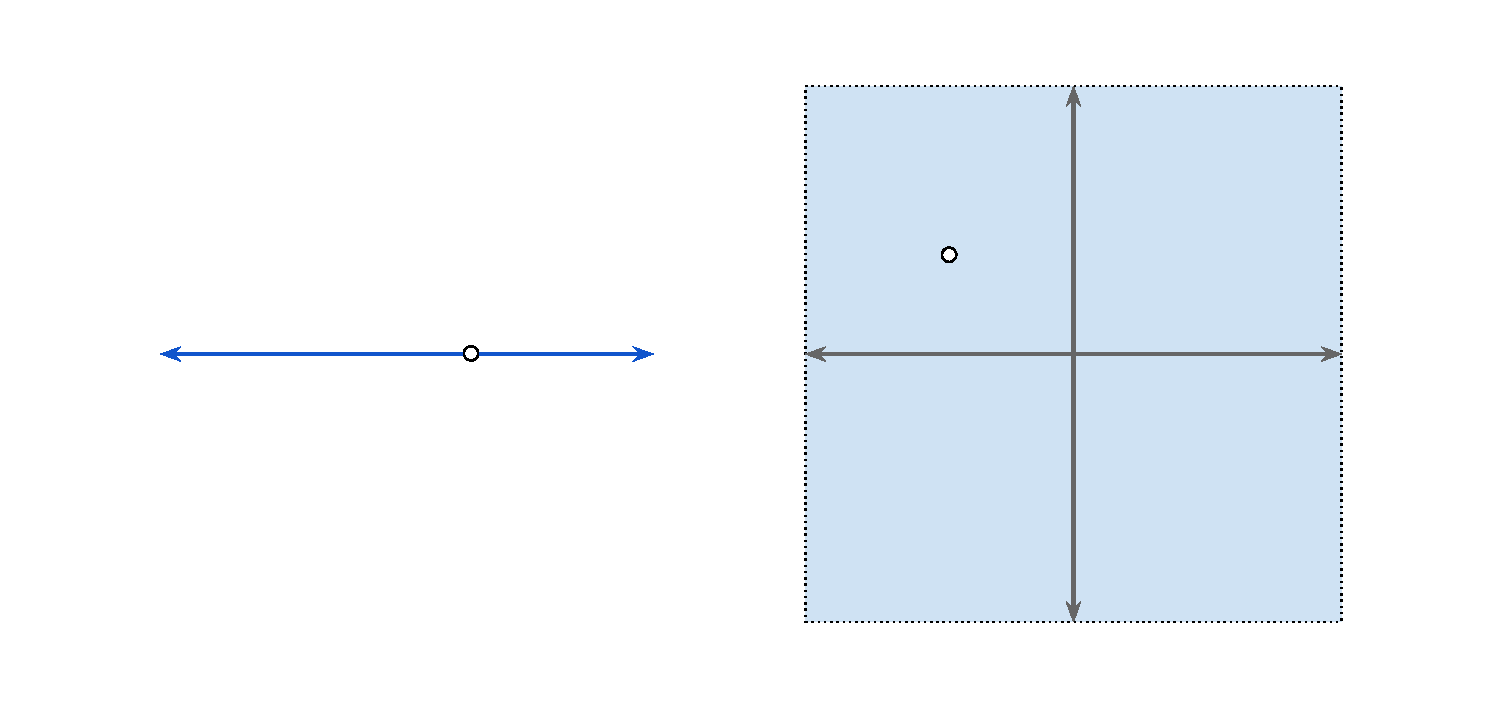
\includegraphics[height=4cm]{images/r_r2_missing_point}
  \end{center}
\end{frame}

\begin{frame}{Why study Topology?}
  \begin{itemize}
    \item 
      One of the primary uses of topology is as a toolkit for other mathematicians. Topological facts are often cited within proofs in other mathematical fields.
  \end{itemize}
  \textbf{Fundamental Theorem of Algebra:} Every polynomial $p(z)$ of degree $n$ has at least one complex root.

  \textit{Trick for Proof:} Compare the topological winding numbers of the curves $q_0(t) = p(0) \not= 0$ and $q_n(t) = p(Re^{2\pi i t}) \not= 0$ around the origin $0+0i$.
\end{frame}
\begin{frame}
  \begin{itemize}
    \item
      However, topology is also emerging as powerful tool in data analysis.
      \begin{itemize}
        \item A data analysist is given a finite number of data points: ordered lists of numbers ($n$-dimensional vectors).
        \item These points may be embedded in the Euclidean topological space $\mathbb{R}^n$: by defining a tolerance, you can ``connect the dots'' to get a collection of simplices approximating the data source.
      \end{itemize}
  \end{itemize}
  {\tiny See: <http://bit.ly/wVejrq>}
\end{frame}
\begin{frame}
  \begin{center}
    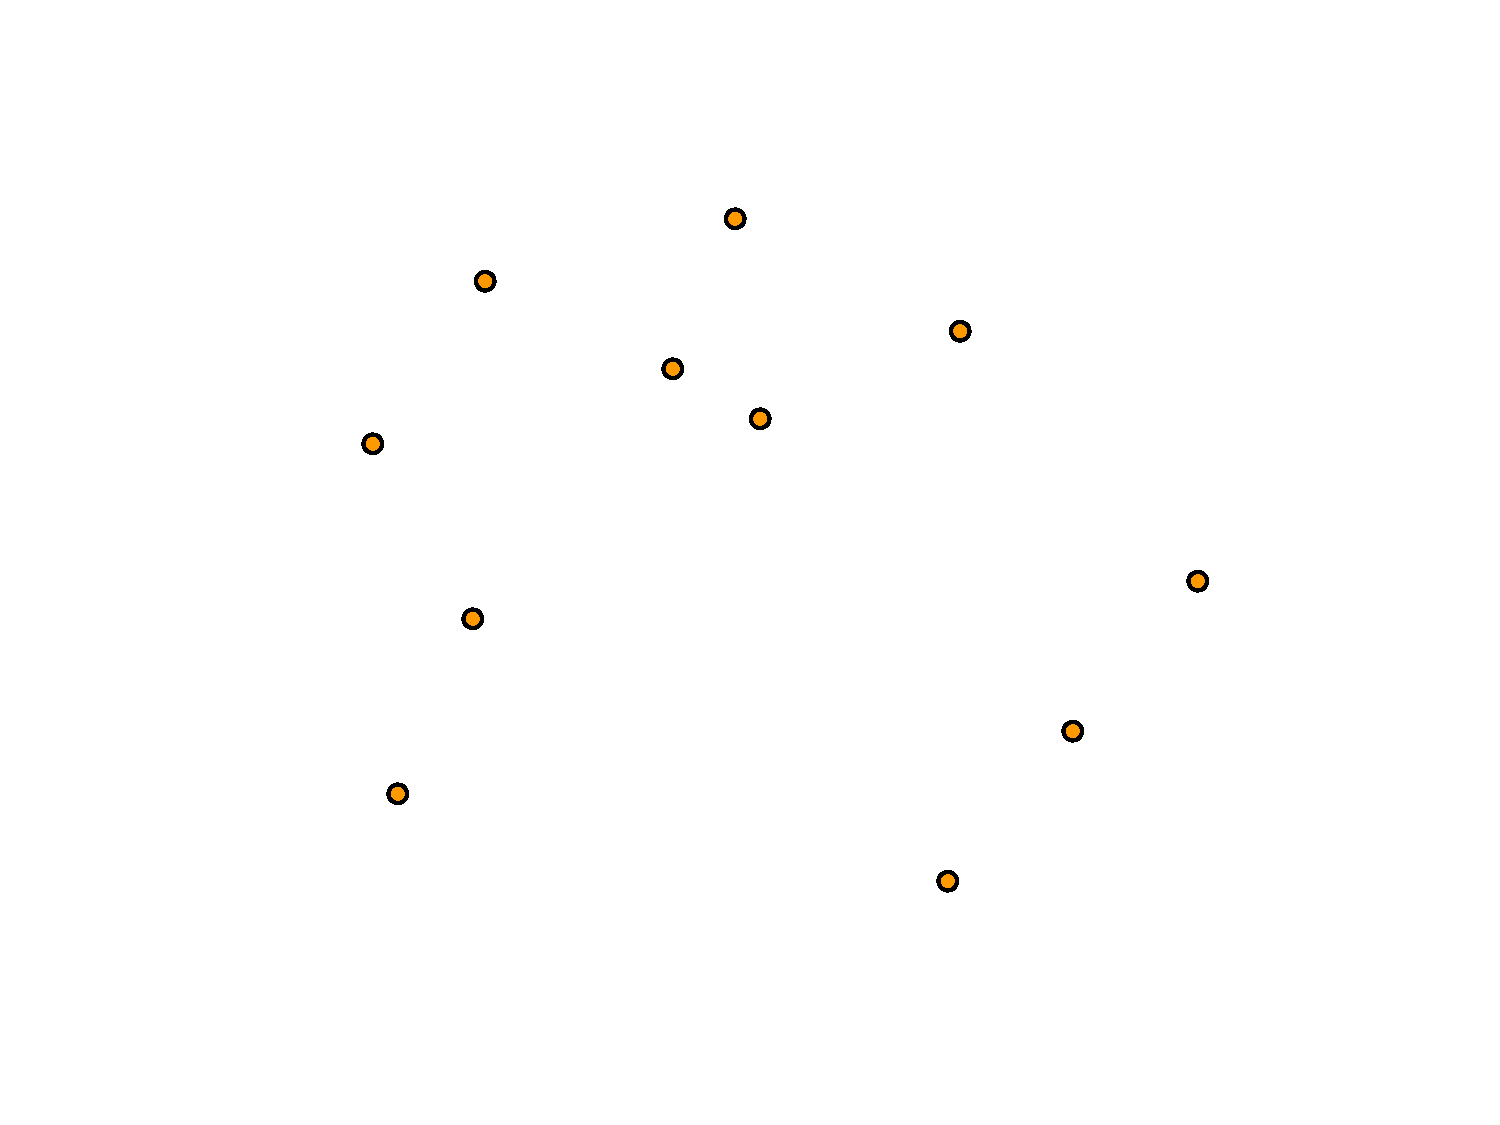
\includegraphics[height=7cm]{images/data_nosource}
  \end{center}
\end{frame}
\begin{frame}
  \begin{center}
    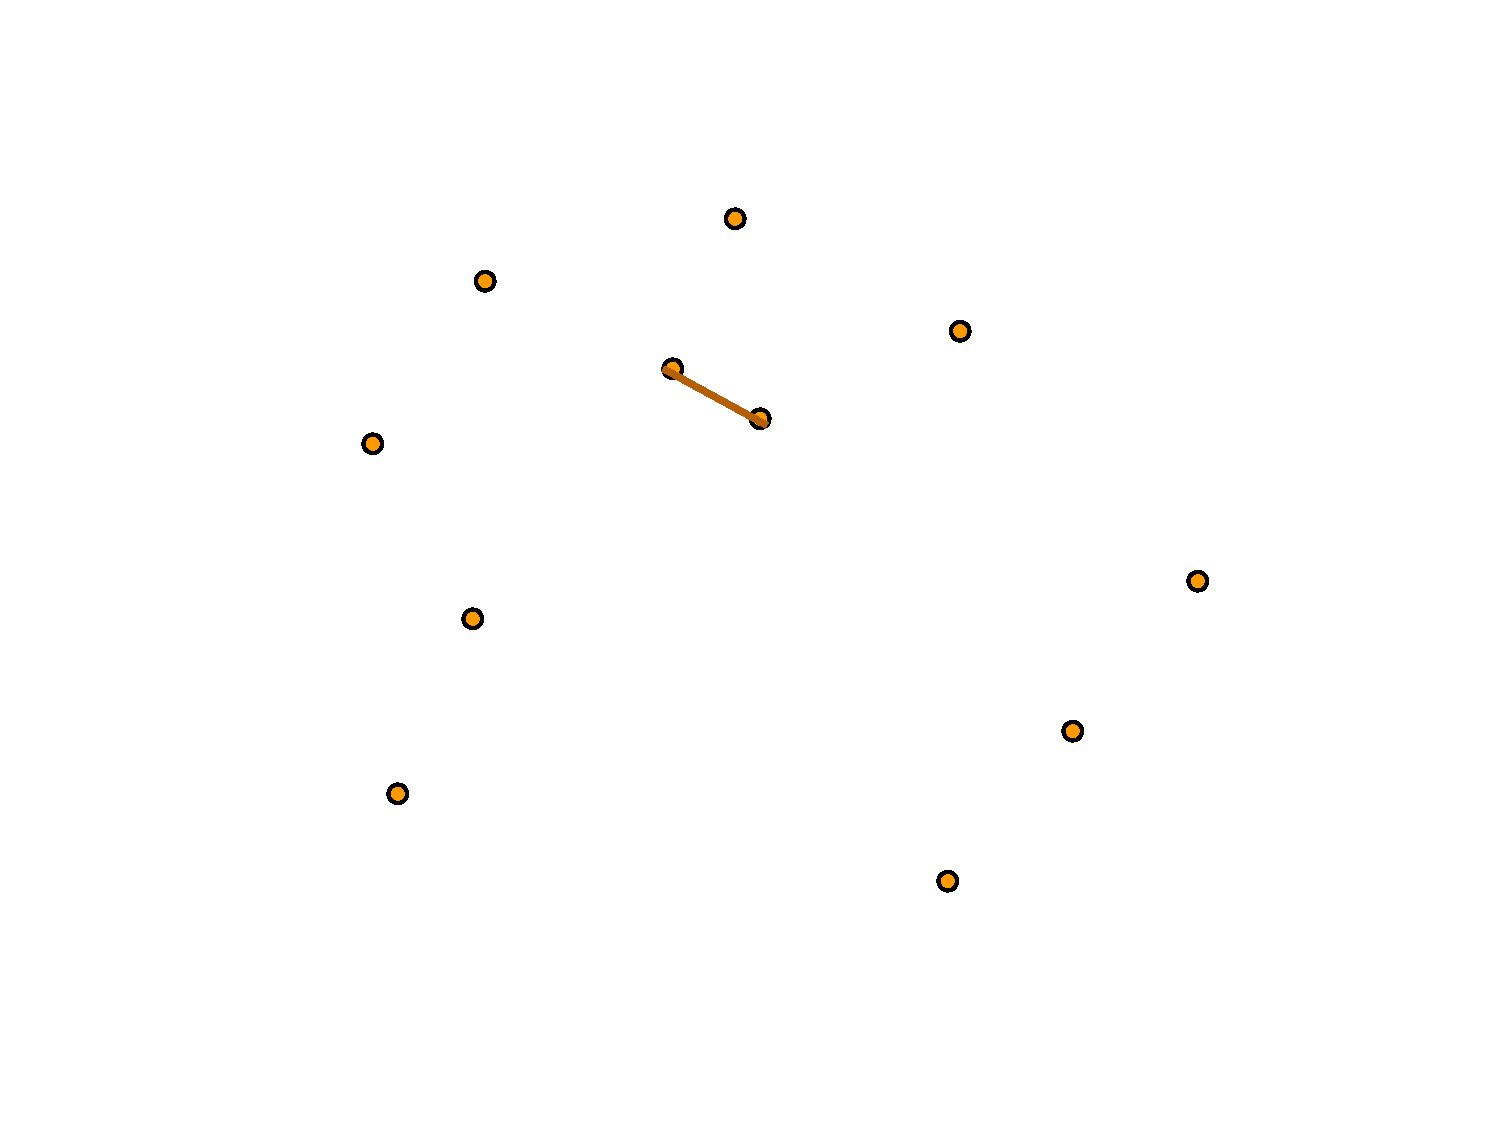
\includegraphics[height=7cm]{images/data_nosource_1}
  \end{center}
\end{frame}
\begin{frame}
  \begin{center}
    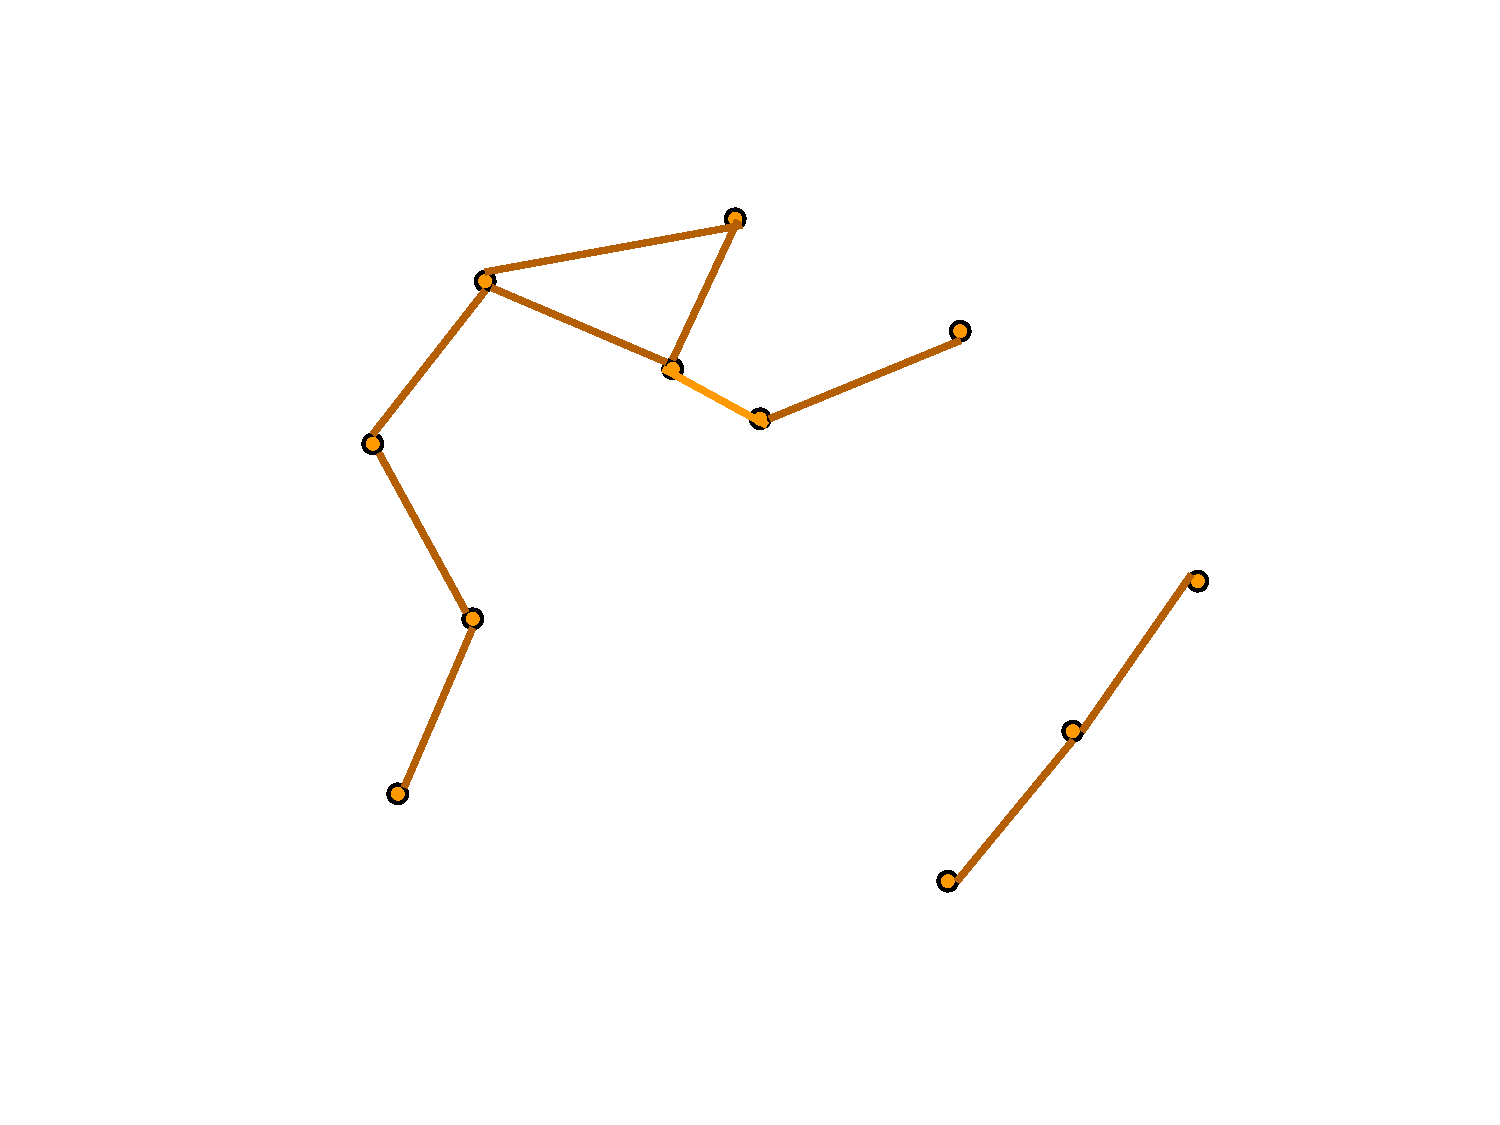
\includegraphics[height=7cm]{images/data_nosource_2}
  \end{center}
\end{frame}
\begin{frame}
  \begin{center}
    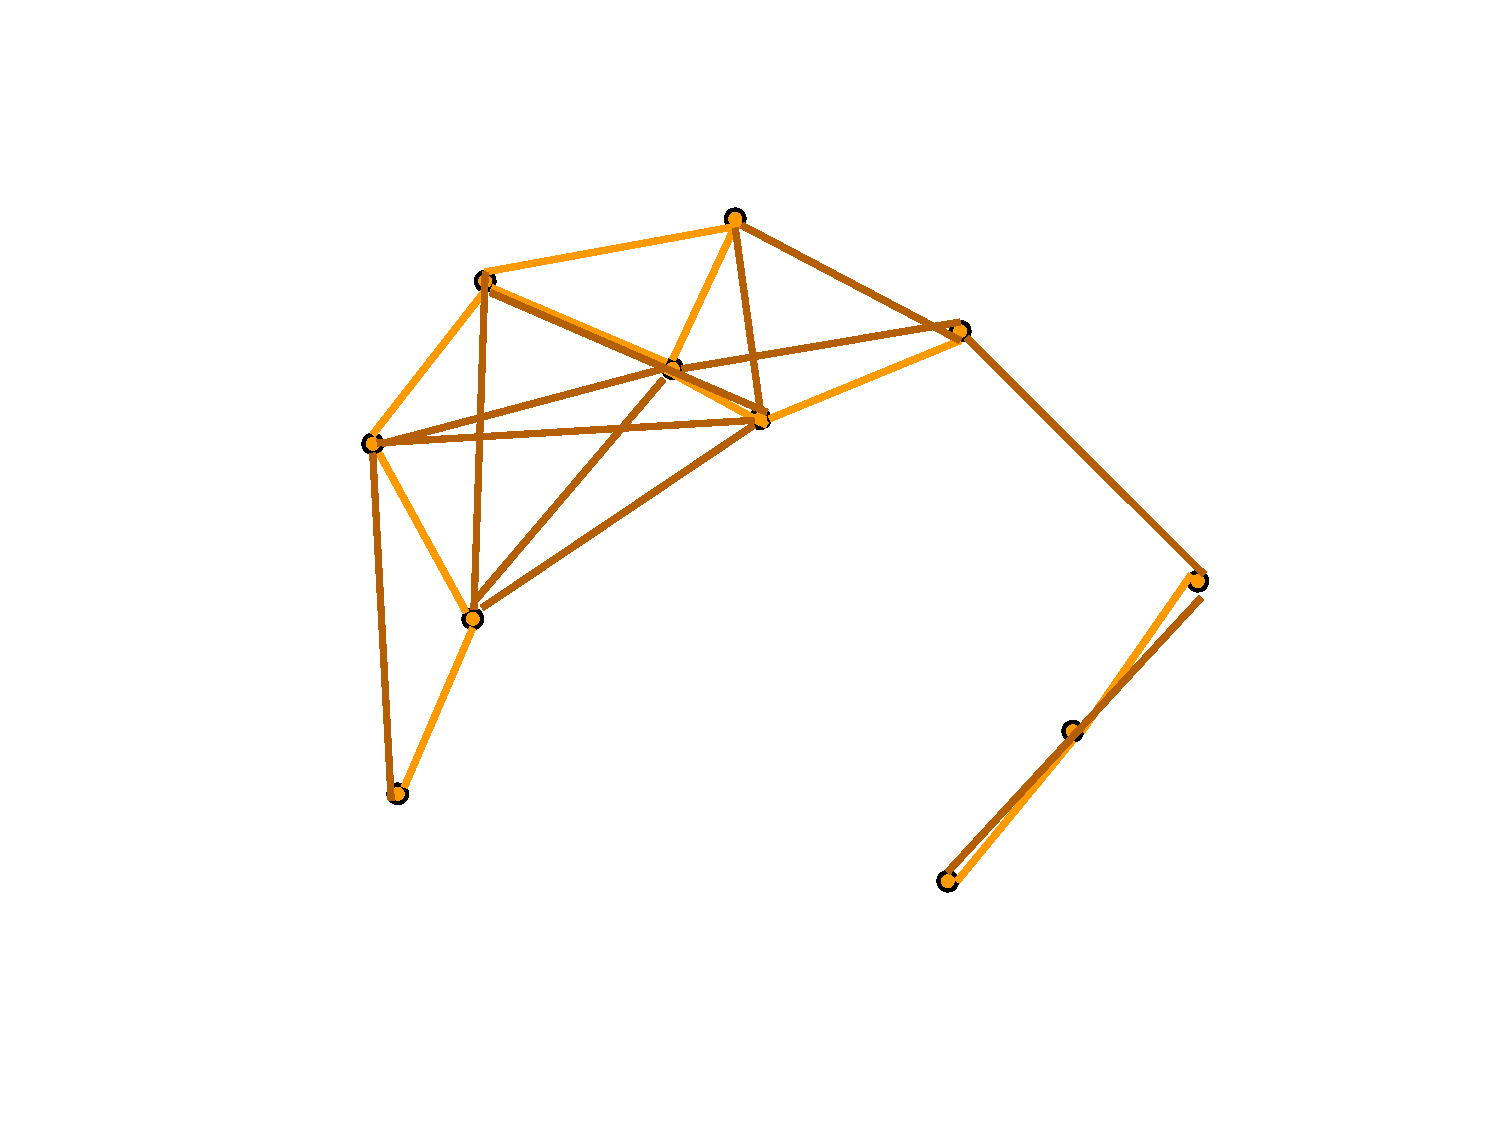
\includegraphics[height=7cm]{images/data_nosource_3}
  \end{center}
\end{frame}
\begin{frame}
  \begin{center}
    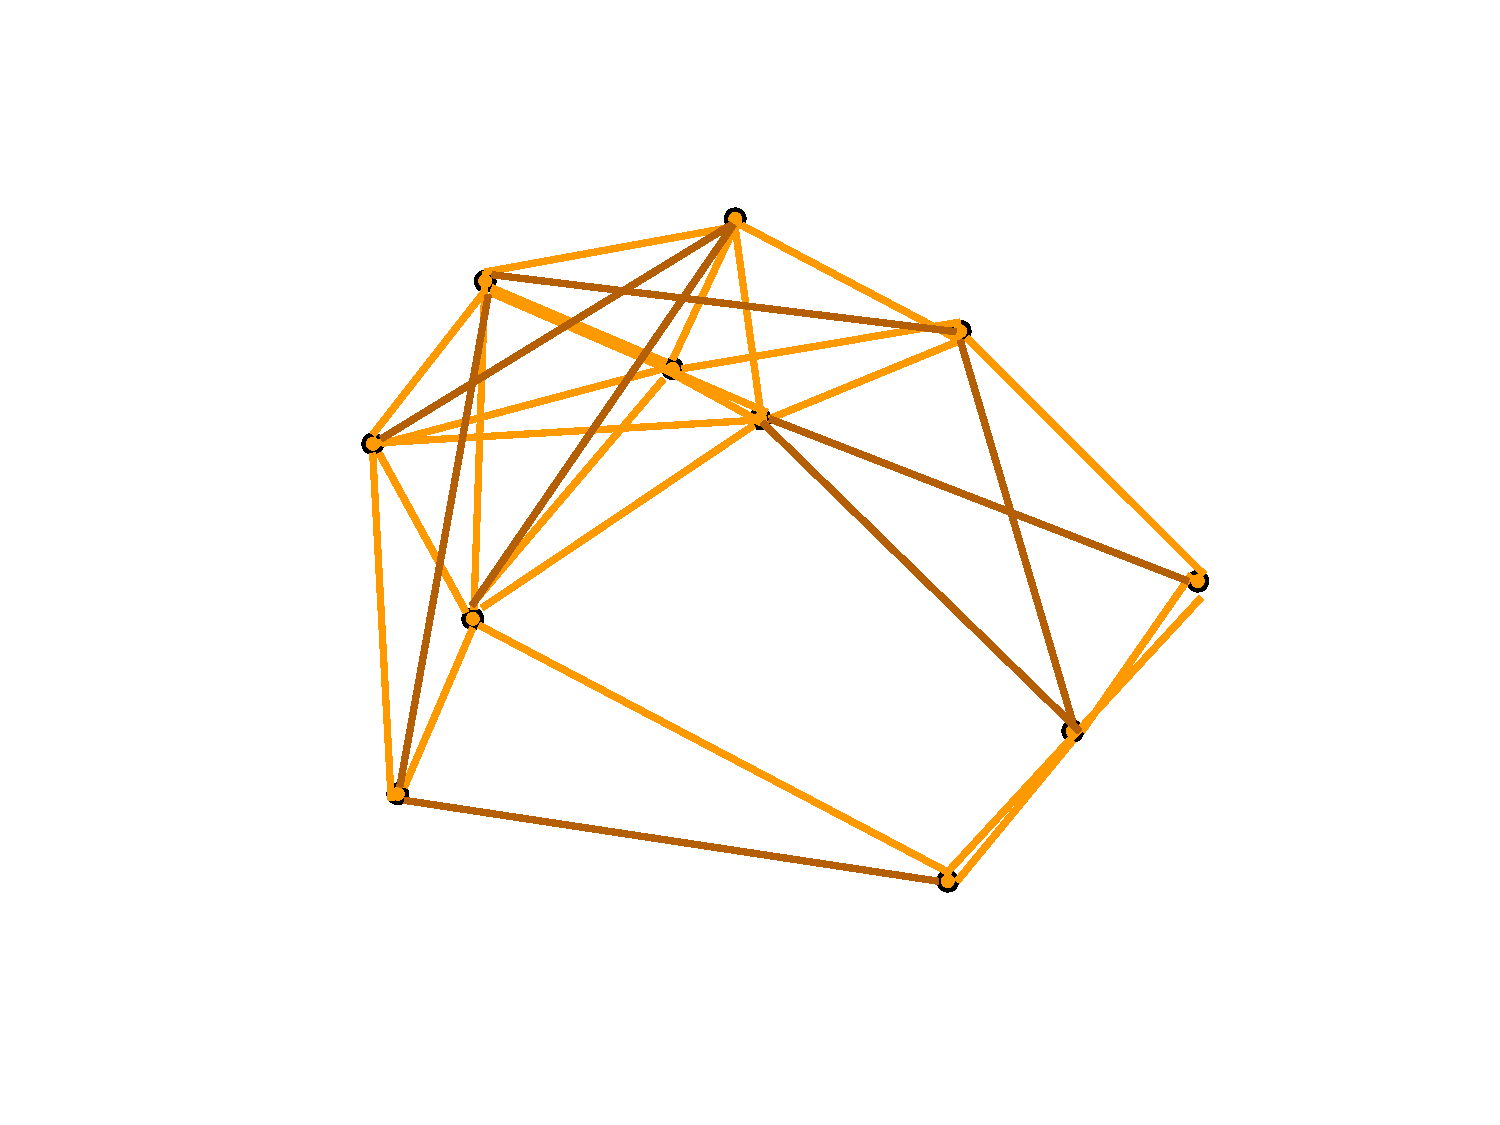
\includegraphics[height=7cm]{images/data_nosource_4}
  \end{center}
\end{frame}
\begin{frame}
  \begin{center}
    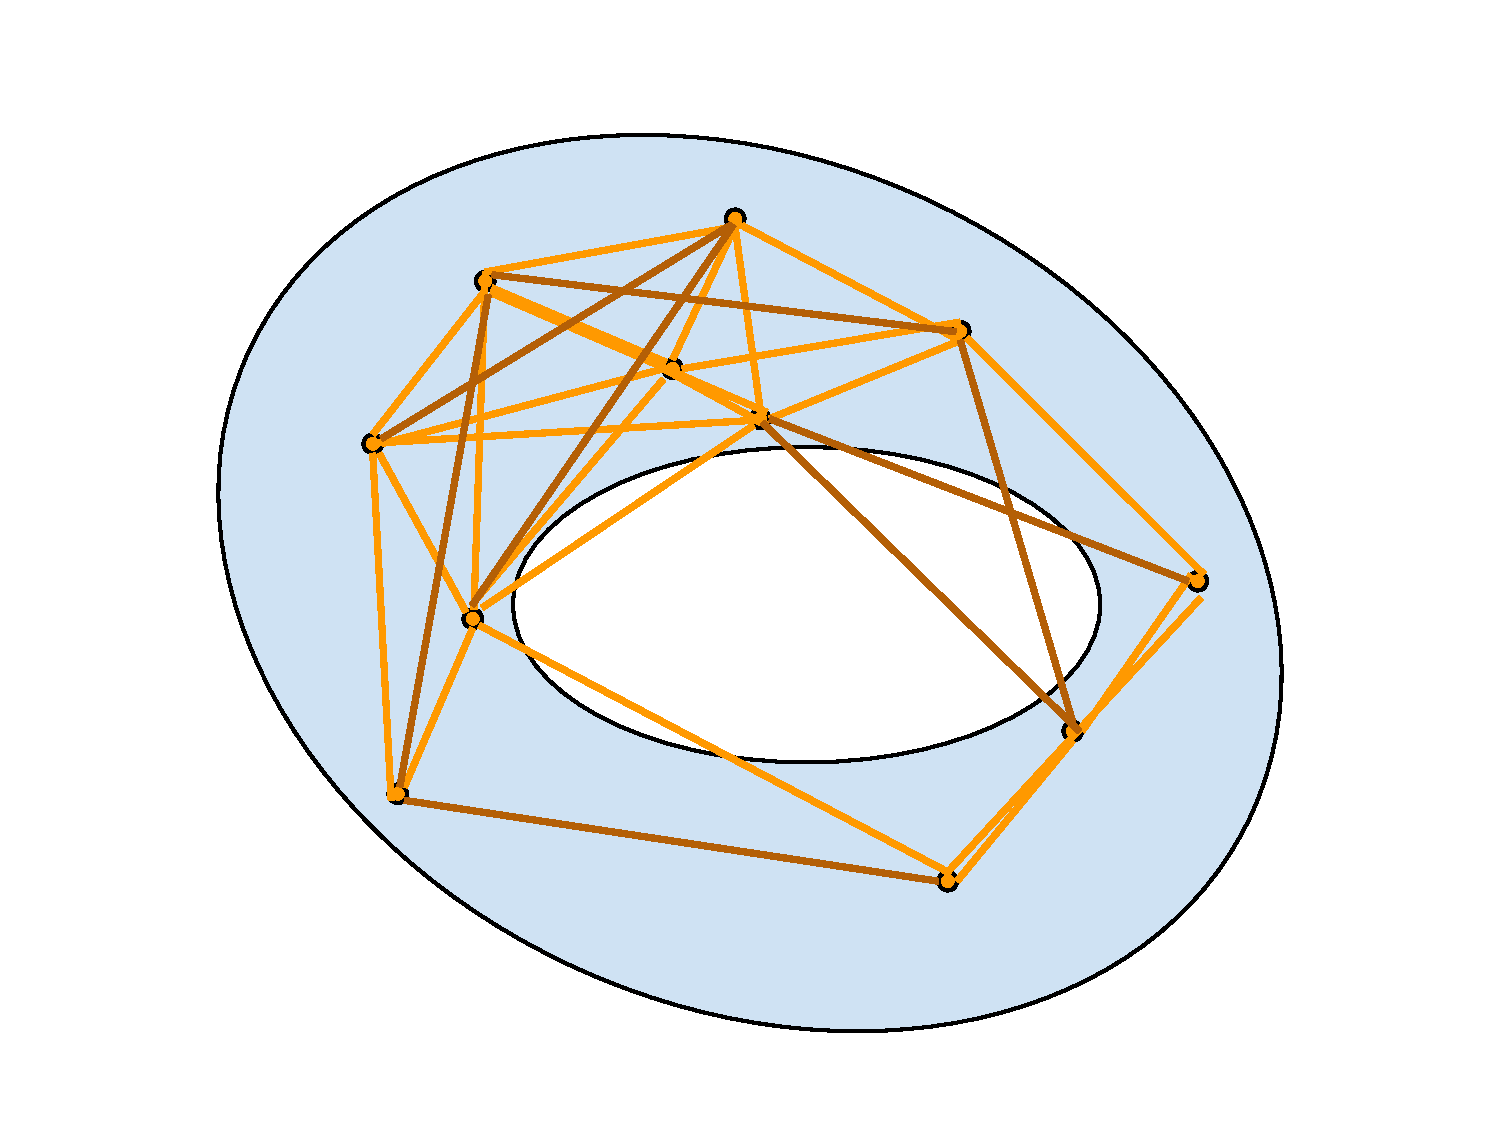
\includegraphics[height=7cm]{images/data_source_4}
  \end{center}
\end{frame}
% \begin{frame}
%   \begin{center}
%     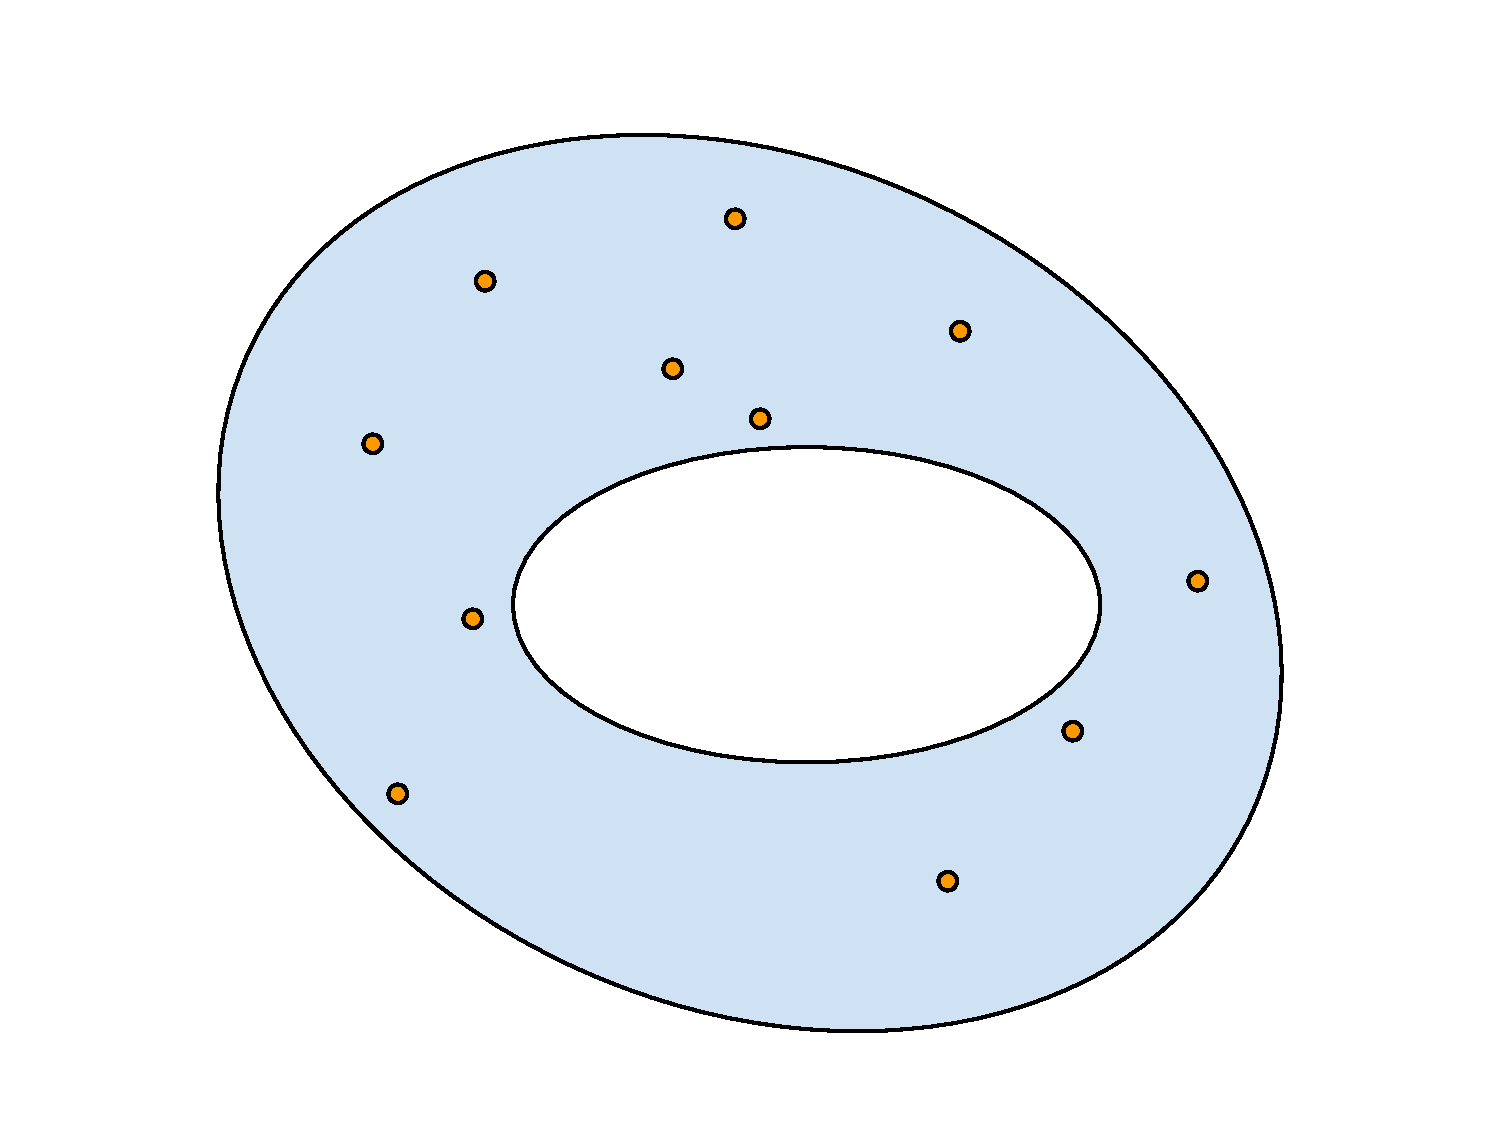
\includegraphics[height=7cm]{images/data_source}
%   \end{center}
% \end{frame}
% \begin{frame}
%   \begin{center}
%     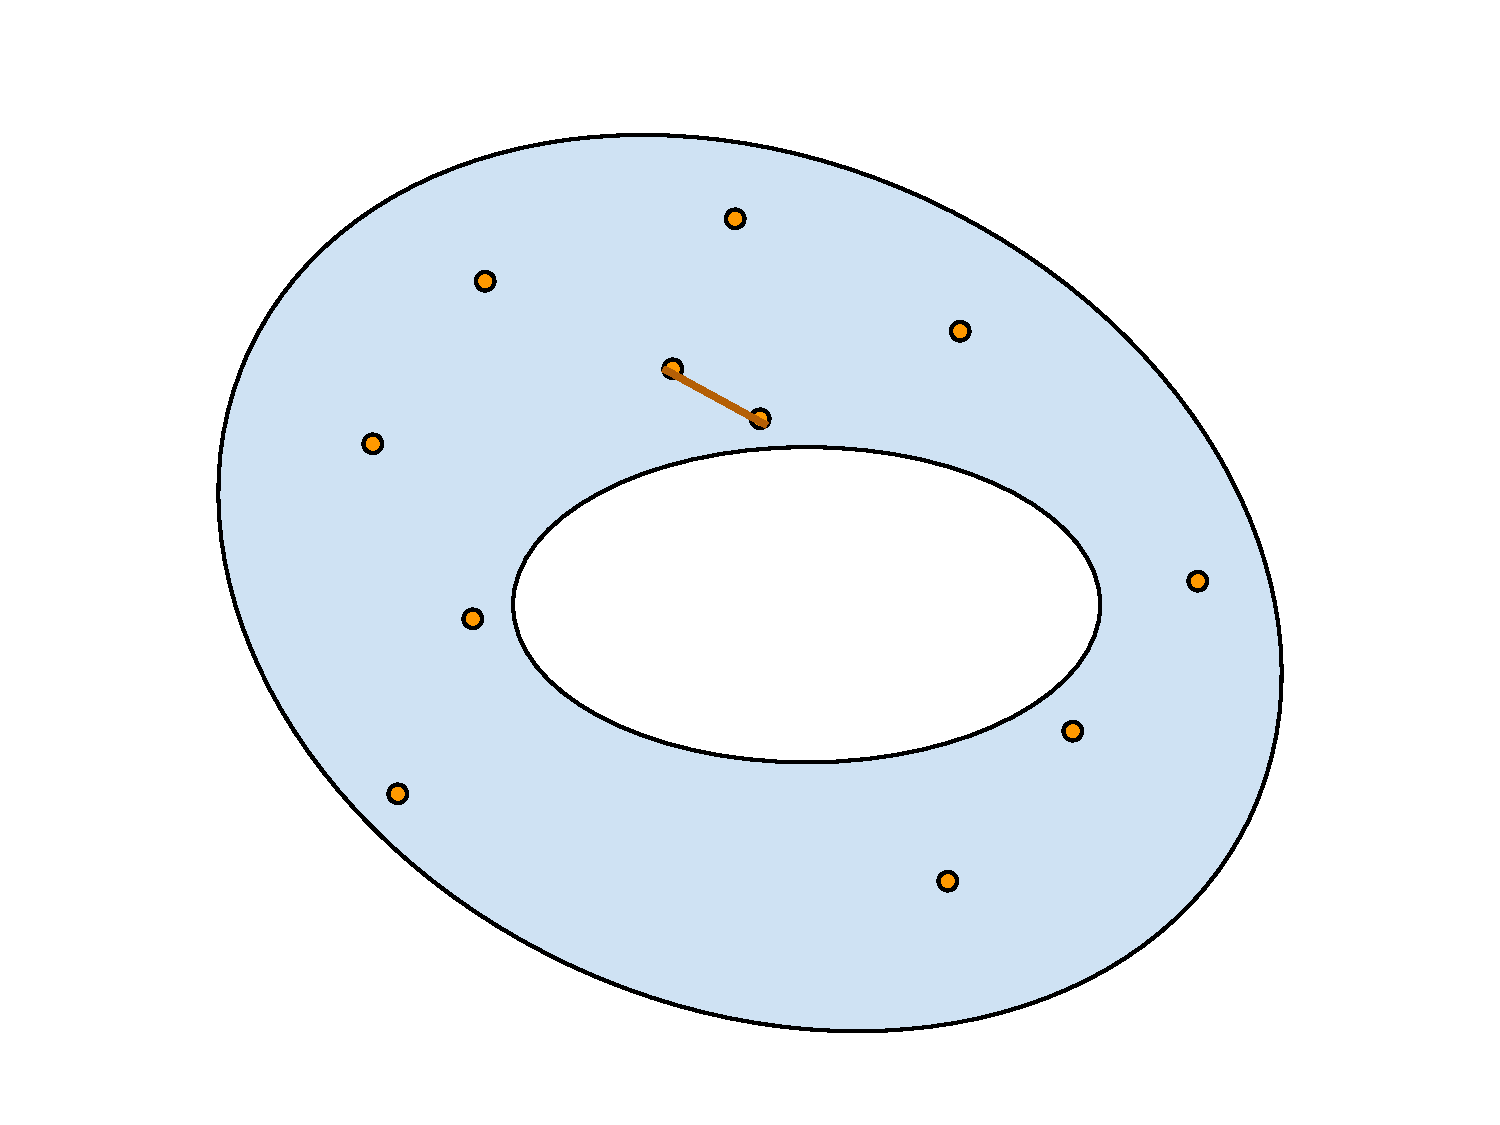
\includegraphics[height=7cm]{images/data_source_1}
%   \end{center}
% \end{frame}
% \begin{frame}
%   \begin{center}
%     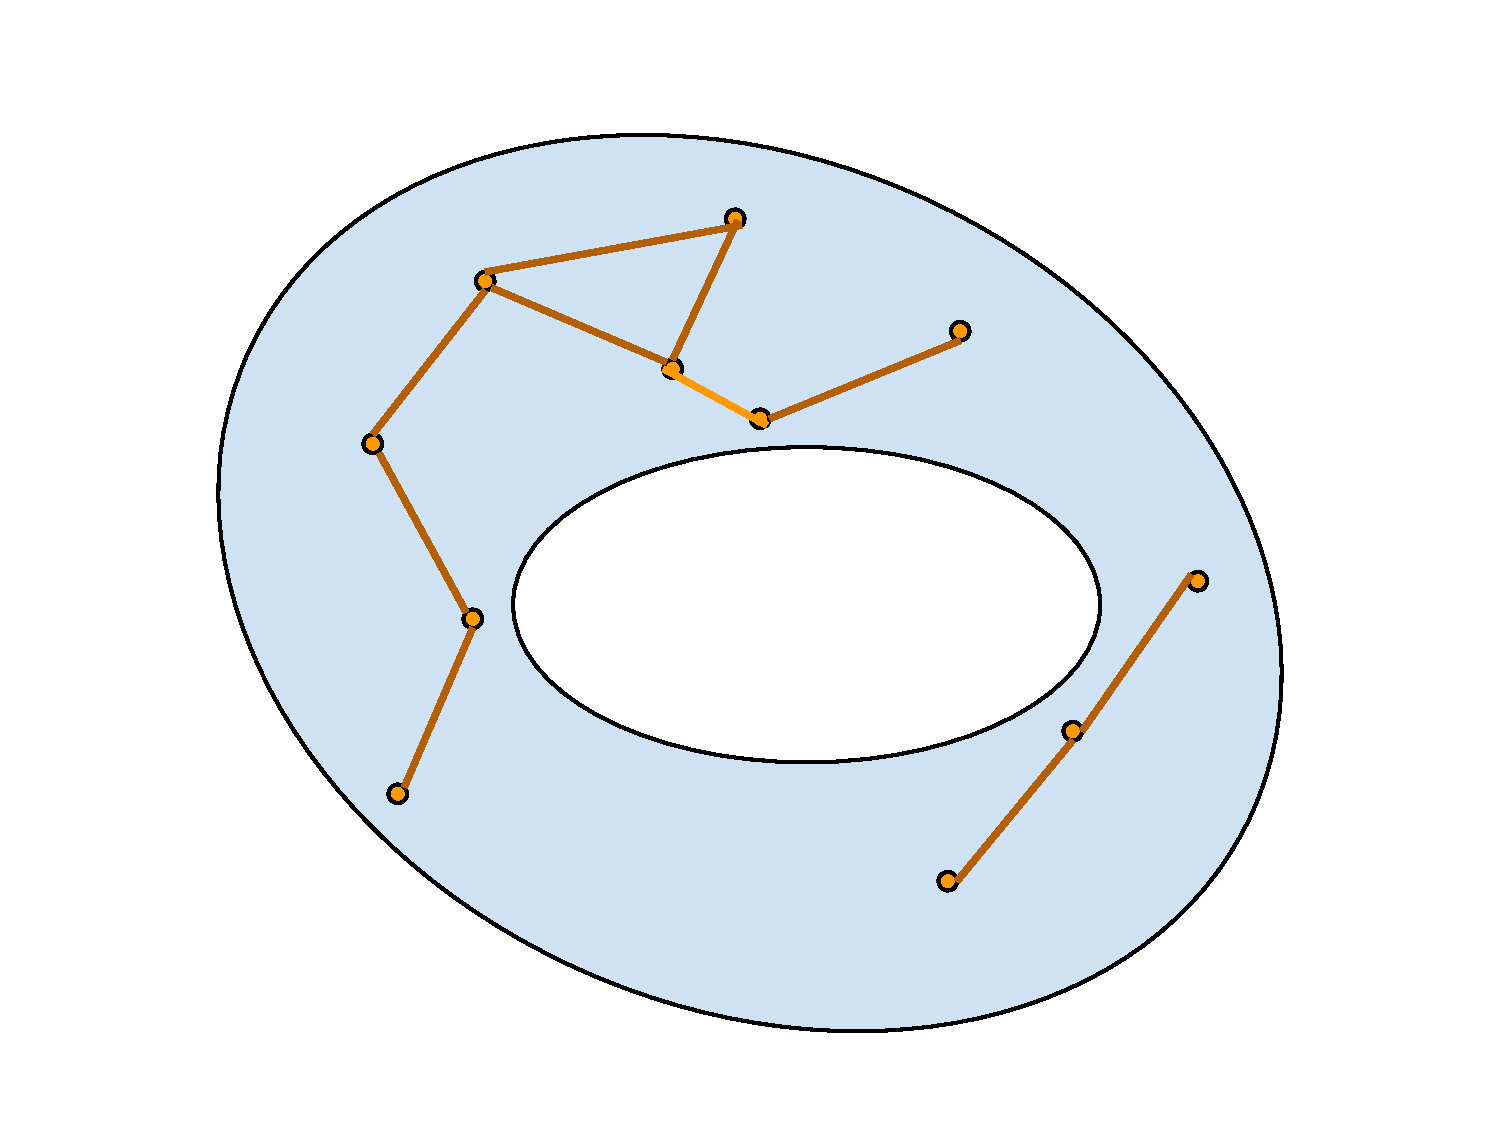
\includegraphics[height=7cm]{images/data_source_2}
%   \end{center}
% \end{frame}
% \begin{frame}
%   \begin{center}
%     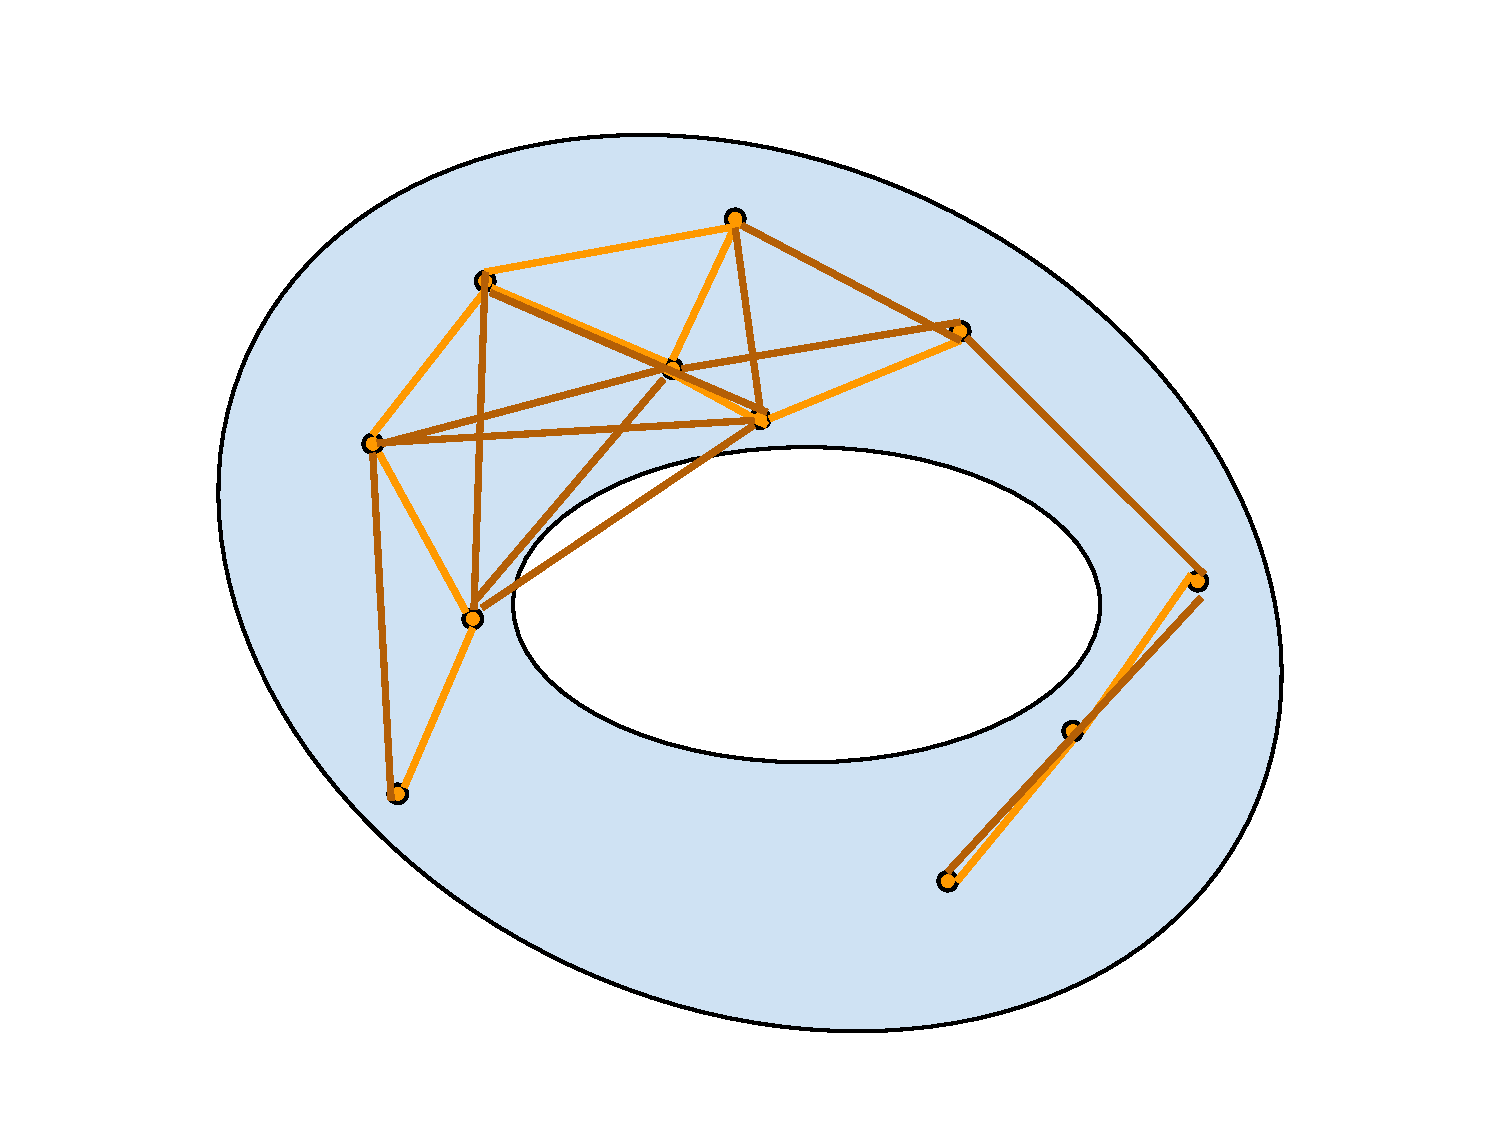
\includegraphics[height=7cm]{images/data_source_3}
%   \end{center}
% \end{frame}
% \begin{frame}
%   \begin{center}
%     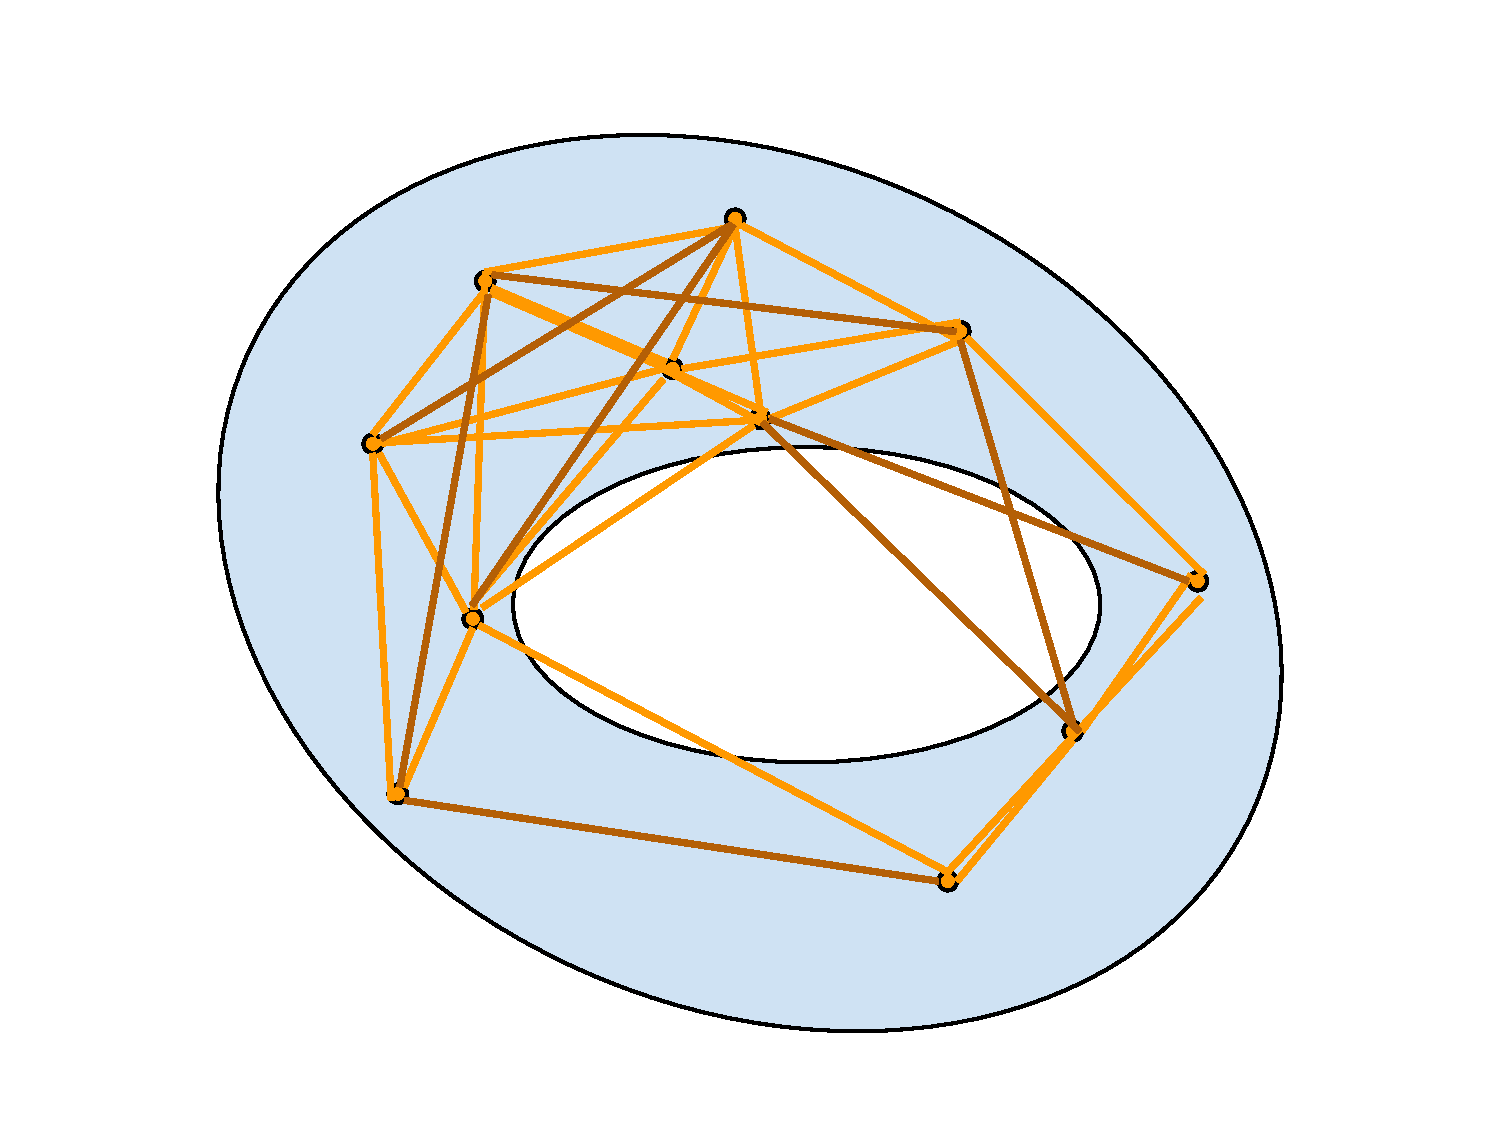
\includegraphics[height=7cm]{images/data_source_4}
%   \end{center}
% \end{frame}

\begin{frame}{What Should I Know?}
  \begin{itemize}
  \item
    For this talk, I'll stick with one familiar topological space and one unfamiliar one.
  \pause
  \item
    When I'm talking about the \textbf{xy-plane}, I'm referring to the usual space of ordered pairs of real numbers from calculus.
  \end{itemize}
  \begin{center}
    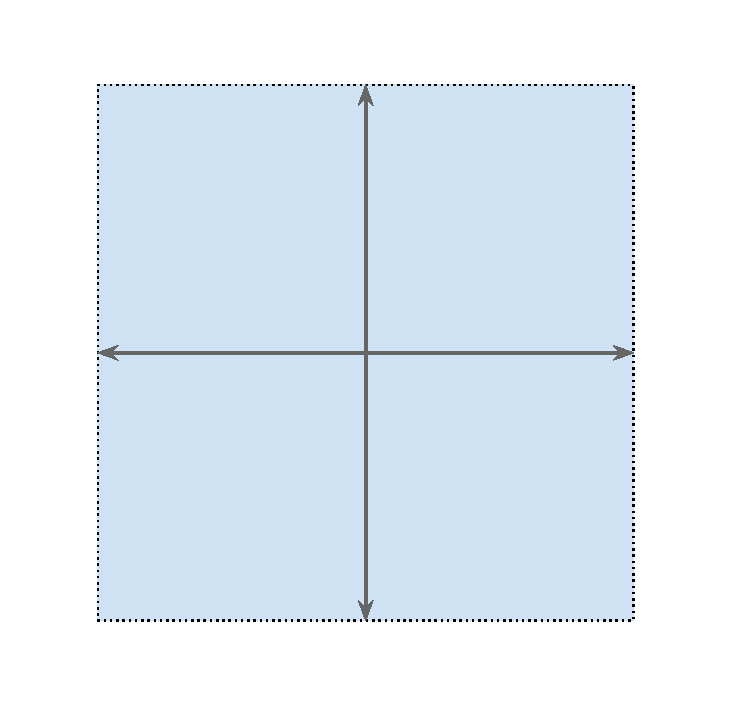
\includegraphics[height=4cm]{images/r2}
  \end{center}
\end{frame}
\begin{frame}
  \begin{itemize}
  \item
    We'll also use another example of a topological space, which I'll call the \textbf{Milky Way space}.
  \end{itemize}
  \begin{center}
    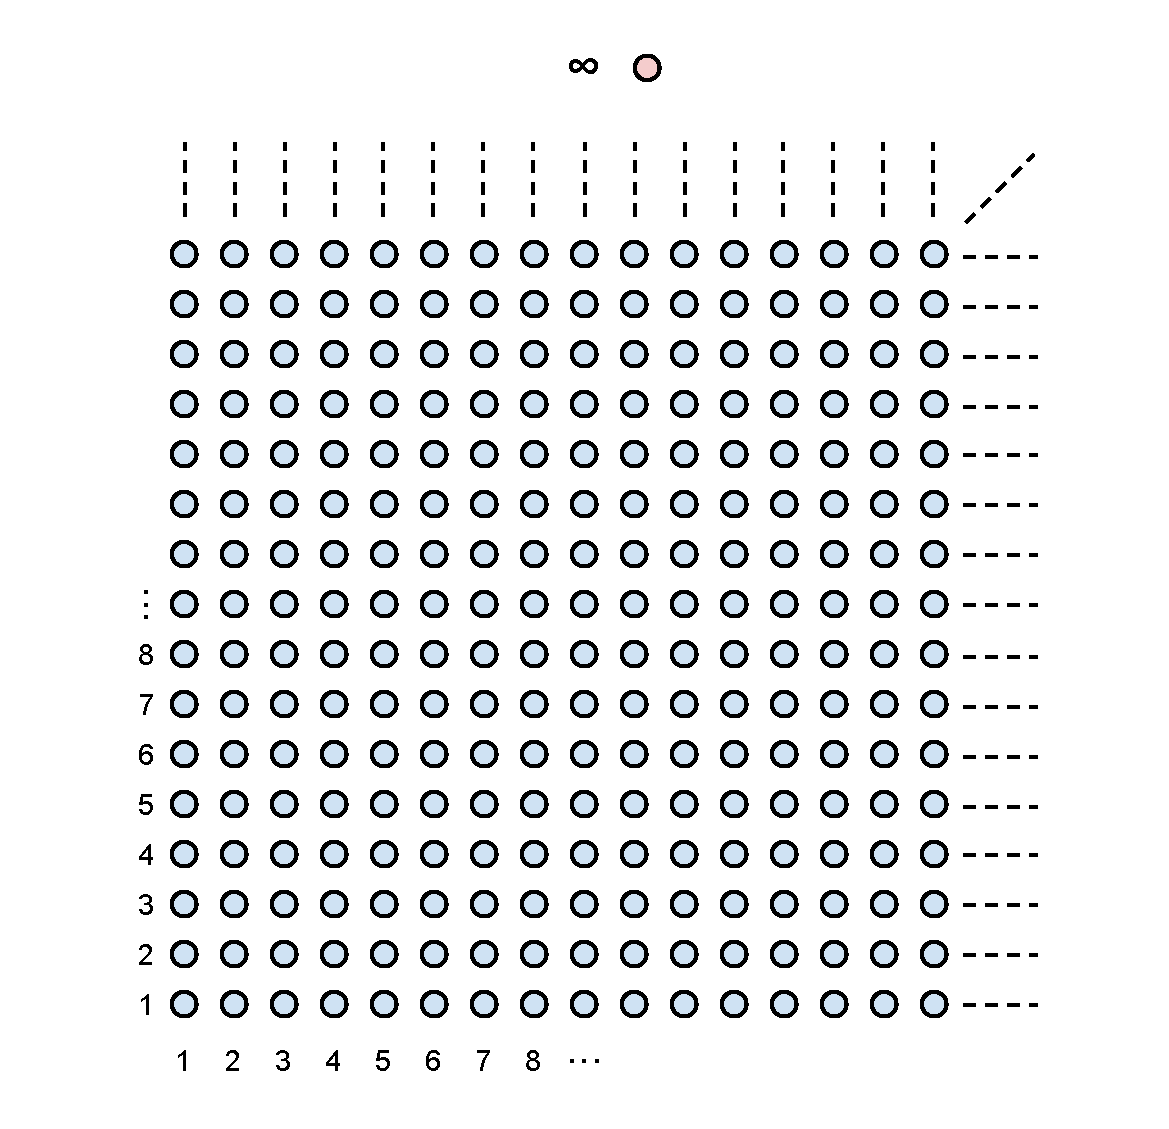
\includegraphics[height=5cm]{images/milky_way}
  \end{center}
  {\tiny See \textit{Katsuya Eda et al, Sequential fans in topology} <http://bit.ly/X6WpQm>}
\end{frame}

\subsection{Games}

\begin{frame}{What's Game Theory?}
  \begin{itemize}
  \item
    Game theory is a powerful tool of use to anyone interested in the study of strategic decision-making: economists, biologists, logicians, political scientists...
  \pause
  \item
    Within game theory, there are two main types of two-player games: \textbf{simultaneous} and \textbf{sequential}.
  \end{itemize}
\end{frame}
\begin{frame}
  \begin{itemize}
  \item
    Simultaneous games include the famous \textbf{Prisoner's Dilemma}: should a prisoner testify against his partner in exchange for a light sentence, knowing that his partner is simultaneously given the same option?
  \end{itemize}
  \begin{center}
    \includegraphics[height=4cm]{images/prisoners}
  \end{center}
  {\tiny See: <http://bit.ly/XaPSCR>}
\end{frame}

\begin{frame}{What's a Sequential Game?}
  \begin{itemize}
  \item
    However, my research is concerned with \textbf{sequential games}. Tic-tac-toe and Chess are handy examples we're all familiar with.
  \end{itemize} 
  \begin{center}
    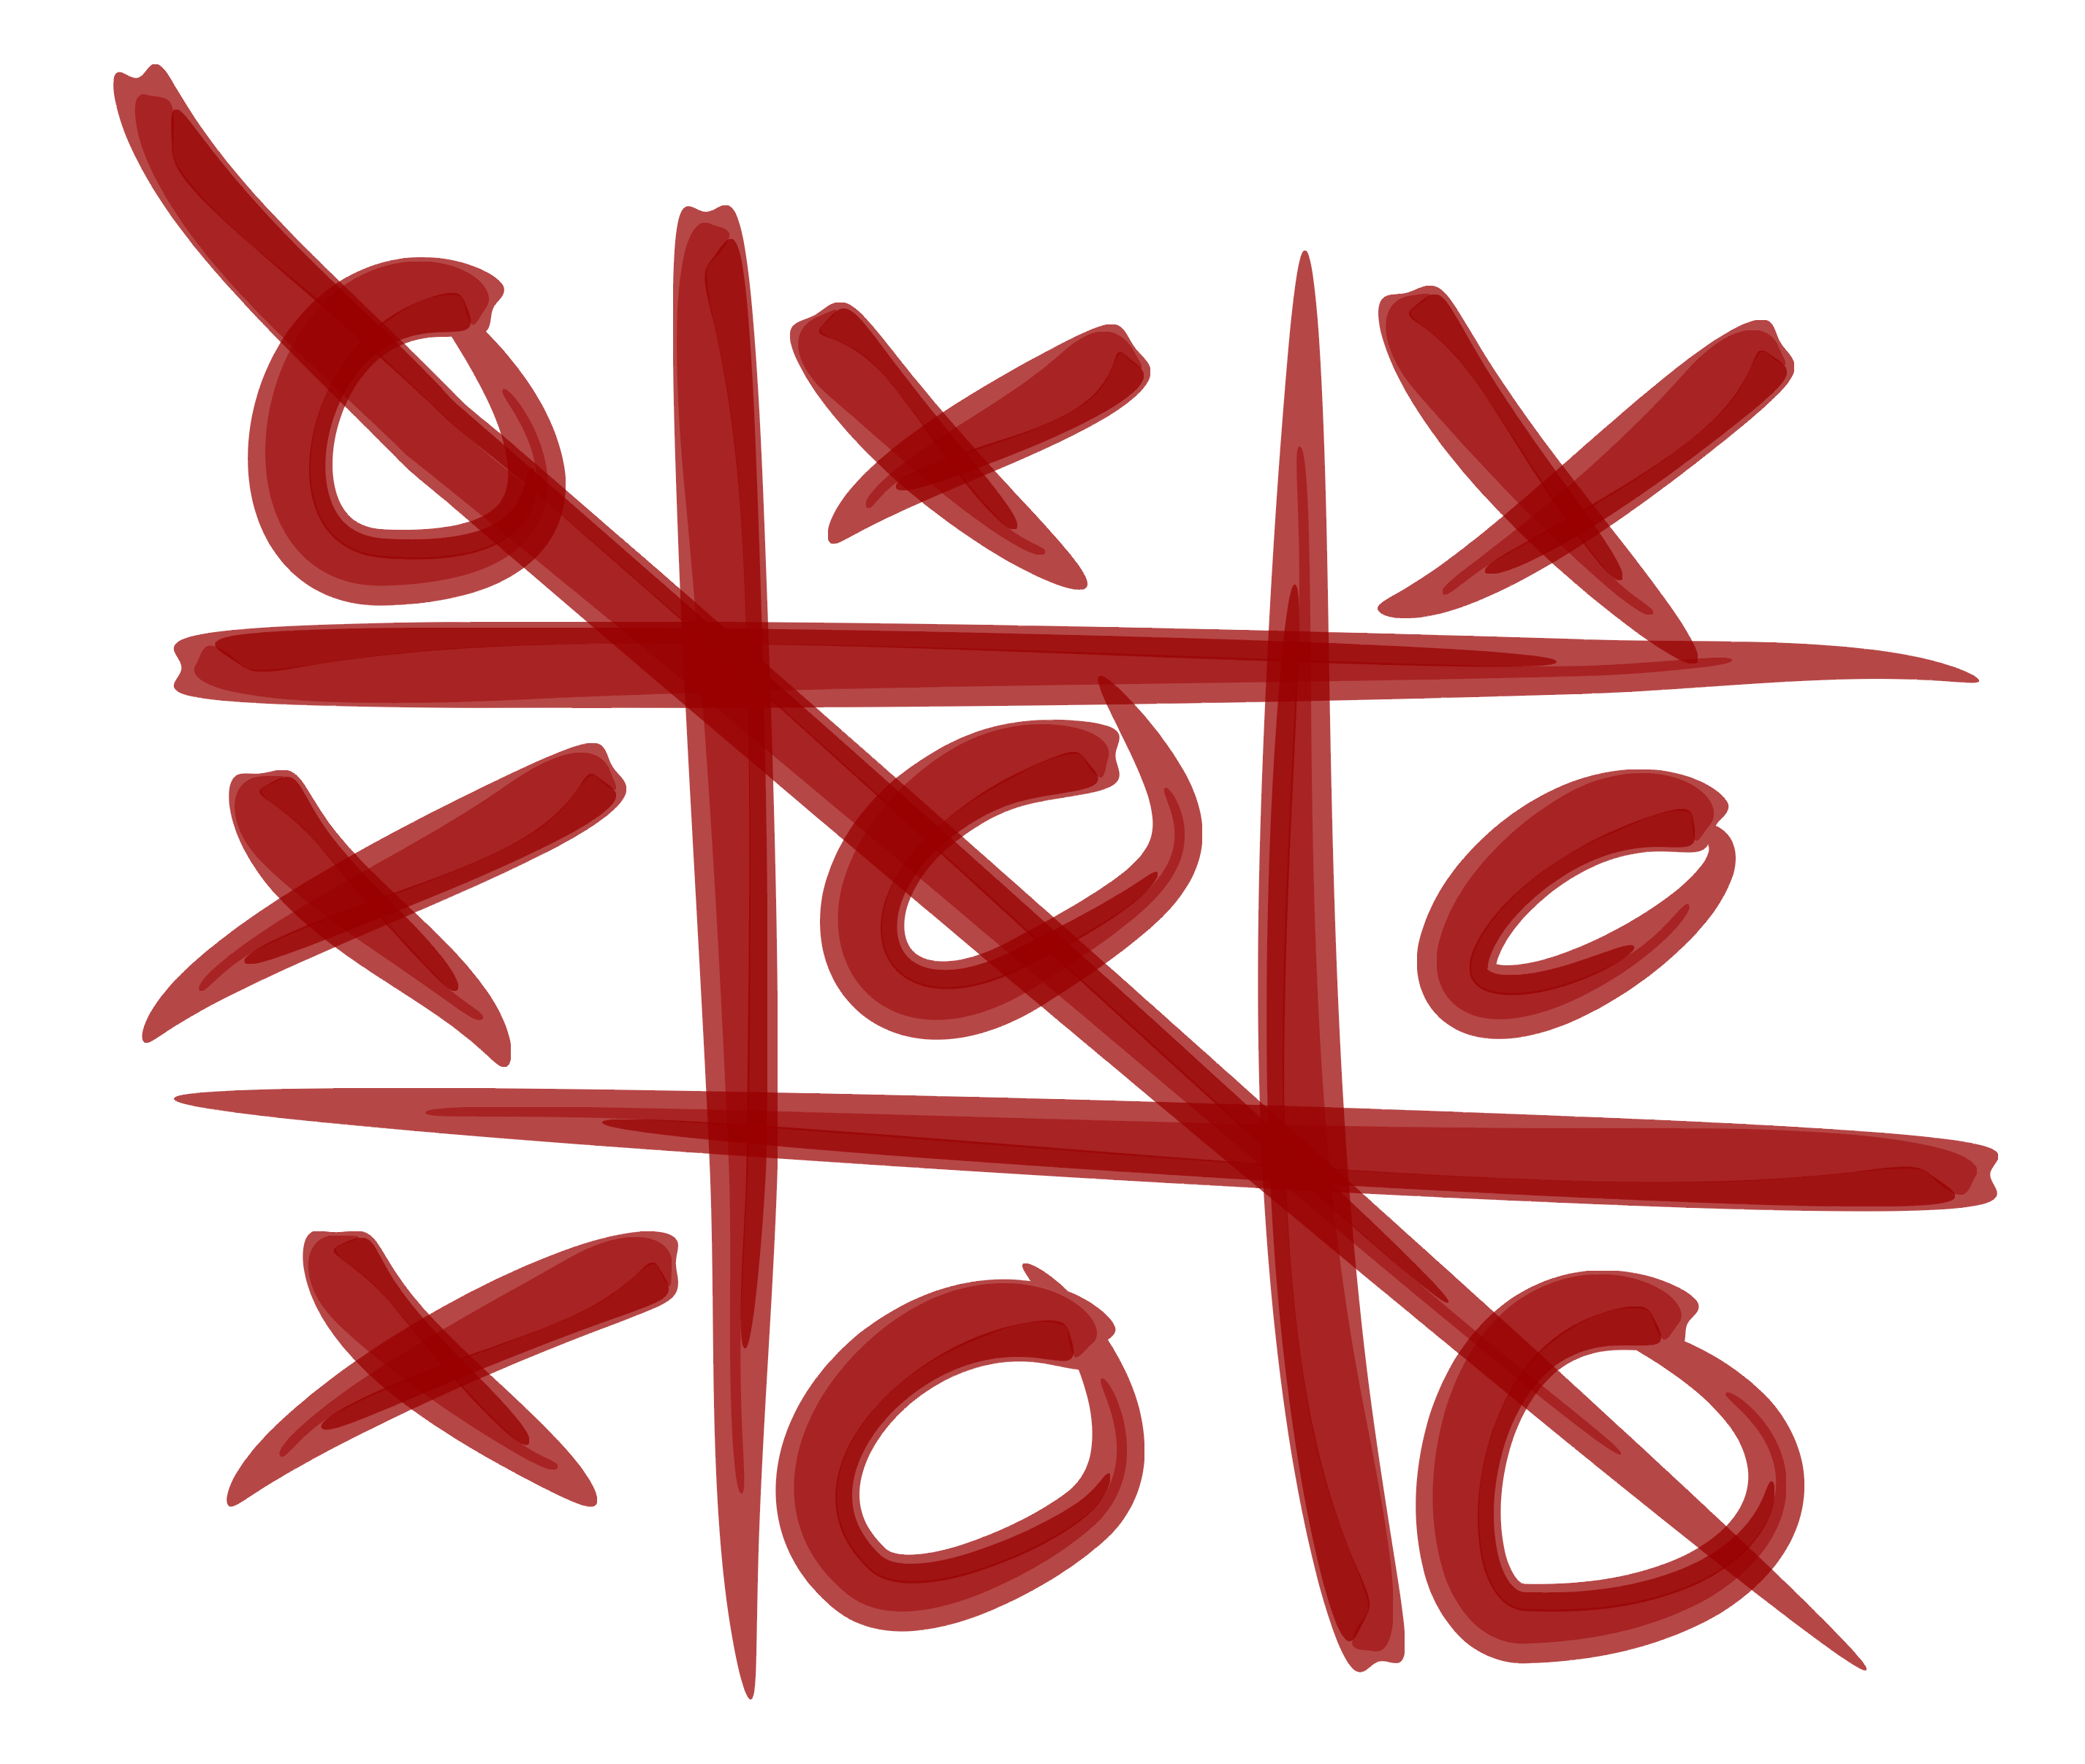
\includegraphics[height=3.5cm]{images/tictactoe}
    \includegraphics[height=3.5cm]{images/chess}
  \end{center}
\end{frame}
\begin{frame}
  \begin{itemize}
  \item
    Mathematically, we can model sequential games by tracking the decisions made by each player during each round.
  \end{itemize}
  \begin{center}
    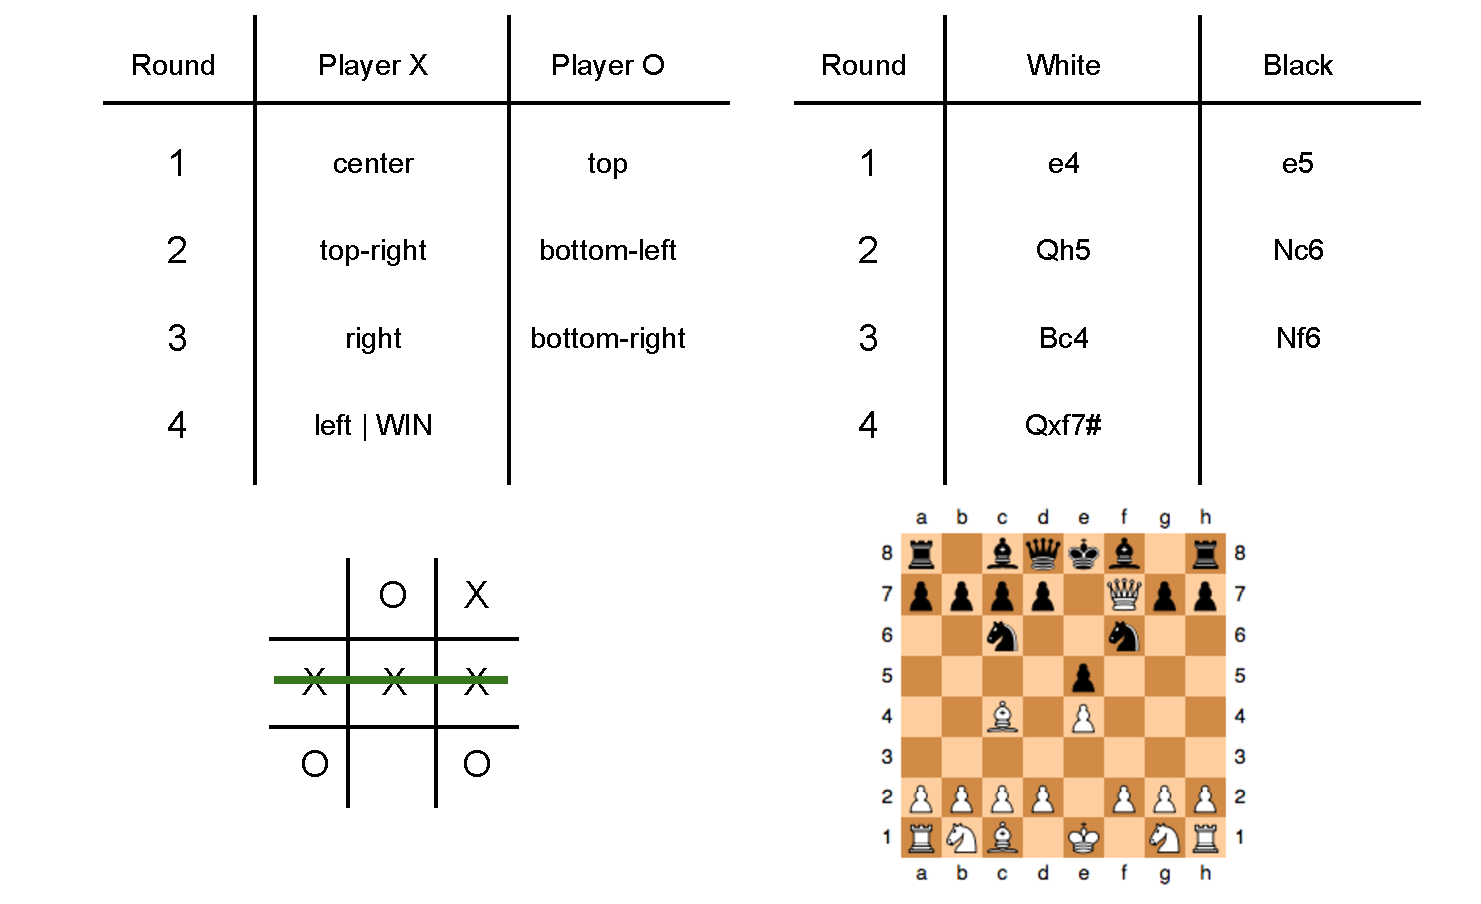
\includegraphics[height=5cm]{images/tictactoe_chess_gameplay}
  \end{center}
\end{frame}

\begin{frame}{And what's this about Infinite-Length Games?}
  \begin{itemize}
  \item
    A good game designer would avoid this, but mathematically we can consider games which aren't required to terminate in a victory for either player after finitely-many moves.
  \pause
  \item
    In that case, the game never ends, but as long as the players involved have a gameplan, we can consider the result of them sticking to their gameplan: the sequence of choices made by each player.
  \pause
  \item
    If the game doesn't end, we'll have a rule to judge how each player did throughout the game, and declare a winner that way.
  \end{itemize}
  {\tiny See: <http://bit.ly/ZF0Hks>}
\end{frame}



% \begin{frame}{So it's sort of like boxing...}
%   \begin{itemize}
%   \item
%     You can think of these games like a \textbf{boxing match} with infinite rounds.
%   \pause
%   \item
%     Each boxer takes turns swinging at each other. If the swing knocks the other guy out, that's a Win by KO.
%   \pause
%   \item
%     If neither boxer manages to KO the other, then we turn to the judges to evaluate based on how they played throughout the entire game. One of the players must get a Win by Decision.
%   \end{itemize}
% \end{frame}

\section{Topological Games}

\begin{frame}{Topological Games}
  
  \begin{itemize}
    \item
      Topological games are infinite-length sequential games ``played upon'' an arbitrary topological space.
    \pause
    \item
      You can think of topological spaces as variant ``game boards'': the rules are always the same, but the available moves depend on the board we're playing on.
  \end{itemize}

\end{frame}

\subsection{Topological Darts in the $xy$-plane}

\begin{frame}{Topological Darts in the $xy$-plane}
  \begin{itemize}
    \item
      Consider a game of ``Topological Darts'' played in the $xy$-plane.
  \end{itemize}
\end{frame}
\begin{frame}
  Player O places a circular dartboard ("\textbf{O}") of any size on the plane so that it covers the point $(0,0)$.
  \begin{center}
    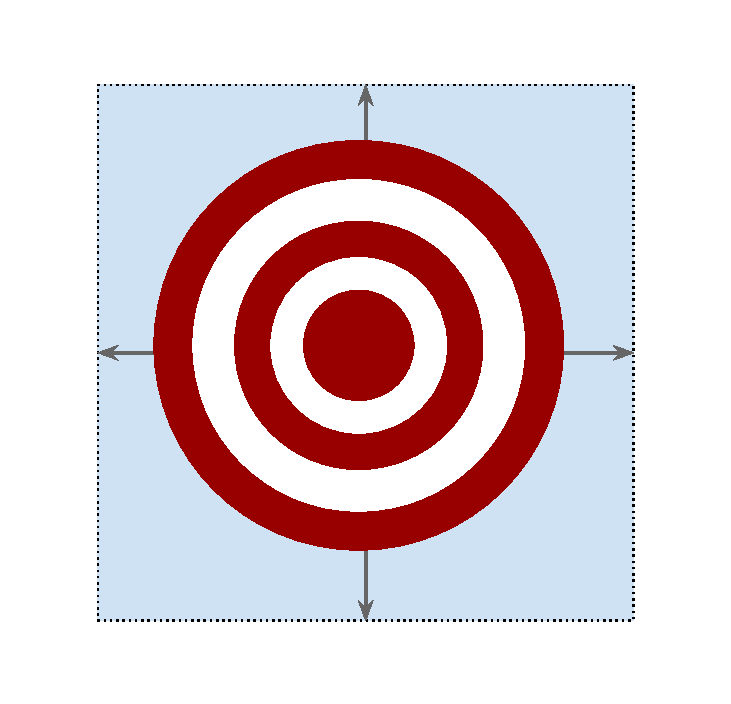
\includegraphics[height=6cm]{images/topdarts_plane_o0}
  \end{center}
\end{frame}
\begin{frame}
  Player P responds by throwing a \textbf{P}ointy dart at the dartboard (picks a point on the plane within the dartboard).
  \begin{center}
    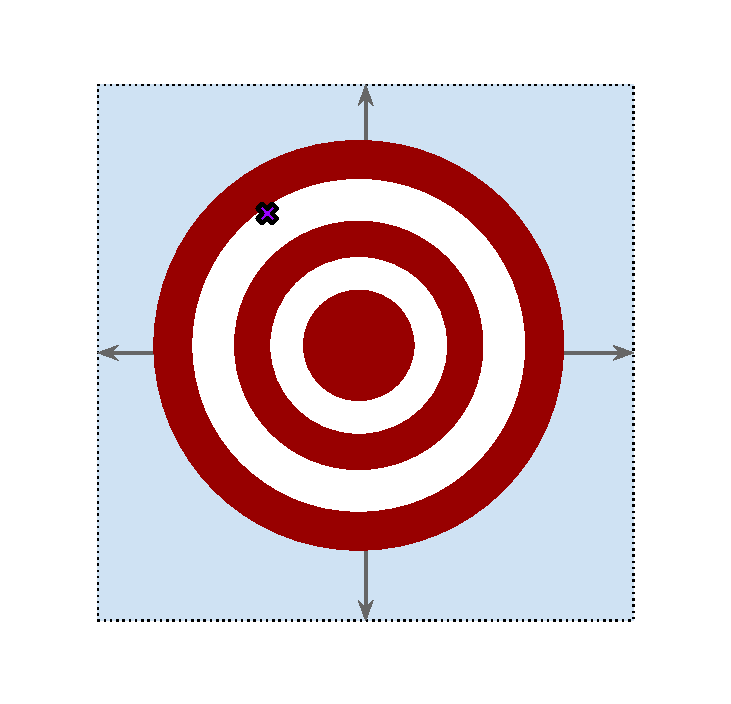
\includegraphics[height=6cm]{images/topdarts_plane_p0}
  \end{center}
\end{frame}
\begin{frame}
  The game continues like this for every round.
  \begin{center}
    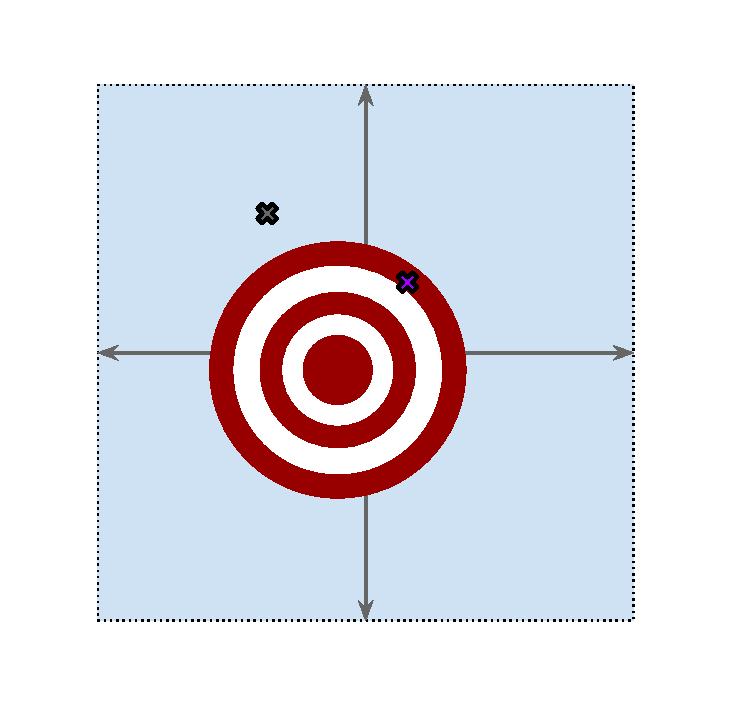
\includegraphics[height=5cm]{images/topdarts_plane_p1}
    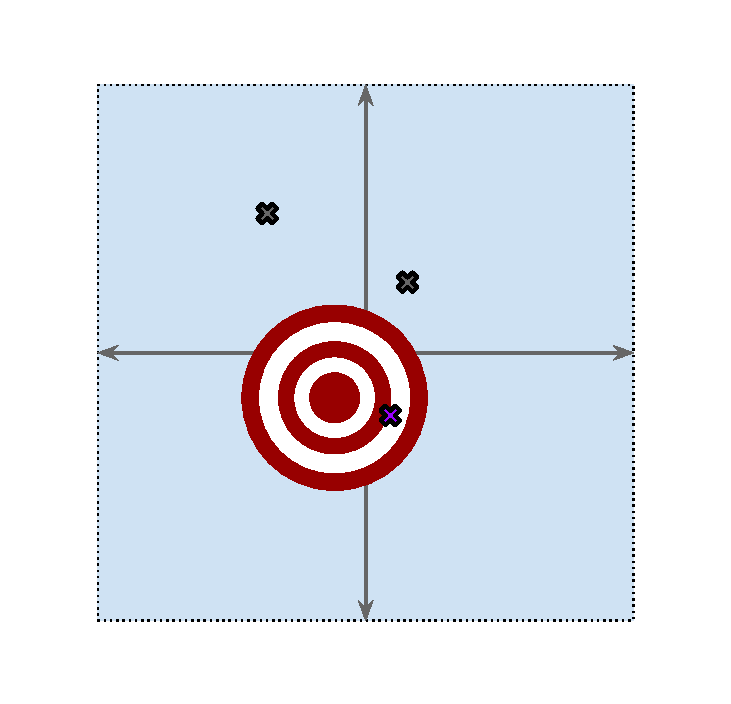
\includegraphics[height=5cm]{images/topdarts_plane_p2}
  \end{center}
\end{frame}

\begin{frame}
  \begin{itemize}
    \item
      Player O automatically wins if Player P ever misses the dartboard.
    \pause
    \item
      Of course, if Player P never misses the dartboard, the game never ends! 
  \end{itemize}
\end{frame}
\begin{frame}
      In that case, if Player P can show a new dartboard covering $(0,0)$ that misses infintely many of the thrown darts, she wins. 
  \begin{center}
    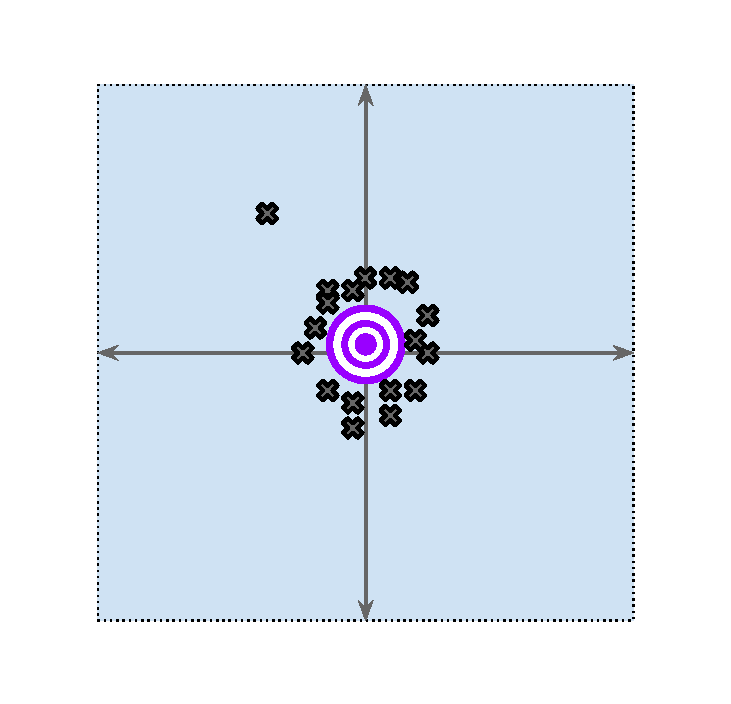
\includegraphics[height=6cm]{images/topdarts_plane_pwins}
  \end{center}
\end{frame}
\begin{frame}
  Otherwise, Player O is the victor. (Since the points \textbf{converge} towards the origin, a dartboard of any size contains all but the first few:)
  \begin{center}
    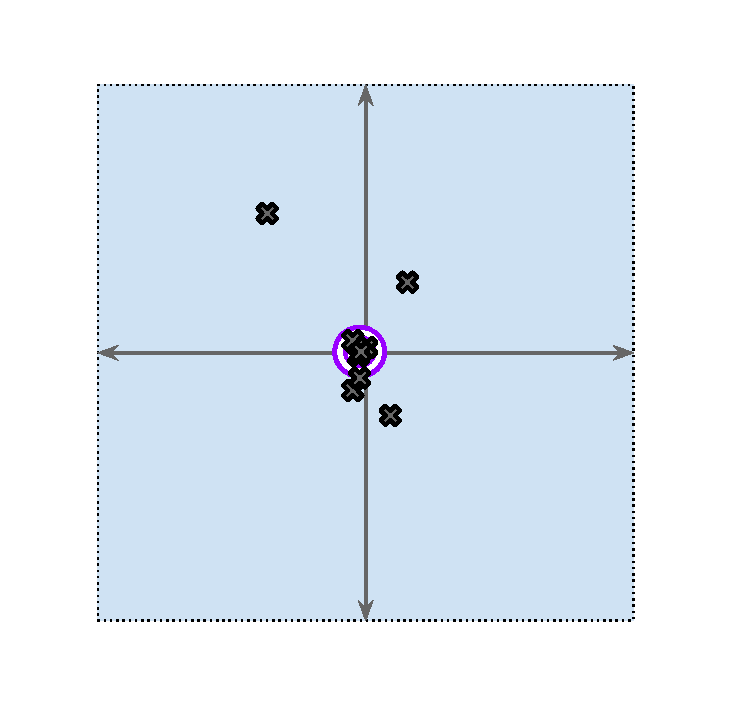
\includegraphics[height=6cm]{images/topdarts_plane_owins}
  \end{center}
\end{frame}

\begin{frame}
  \begin{itemize}
  \item
    Player O has a \textbf{winning (unbeatable) strategy} for Topological Darts when played in the $xy$-plane:
  \end{itemize}
\begin{center}
\begin{tabular}{c|c|c|c}
Round & Board Picker (O) & Dart Thrower (P) & Dist. from $(0,0)$ \\\hline
$1$ & $x^2+y^2 < 1$ & $(x_1,y_1)$ & $< 1$ \\
$2$ & $x^2+y^2 < \frac{1}{4}$ & $(x_2,y_2)$ & $< \frac{1}{2}$ \\
\vdots & \vdots & \vdots & \vdots \\
$n$ & $x^2+y^2 < \frac{1}{n^2}$ & $(x_n,y_n)$ & $< \frac{1}{n}$ \\
\vdots & \vdots & \vdots & \vdots \\
\end{tabular}
\end{center}
\end{frame}

\subsection{Topological Darts in the Milky Way Space}

\begin{frame}{Topological Darts in the Milky Way Space}
  \begin{itemize}
    \item
      Of course, these darts and dartboards are just some glitter and macaroni covering what's really going on mathematically.
    \pause
    \item
      The interior of the circular dartboards in the $xy$-plane represent topological objects known as \textbf{open sets}. What these open sets look like depend on the topological space.
  \end{itemize}
\end{frame}
\begin{frame}
  In our so-called Milky Way Space, the dartboards / open sets placed around the point $\infty$ look like
  \begin{center}
    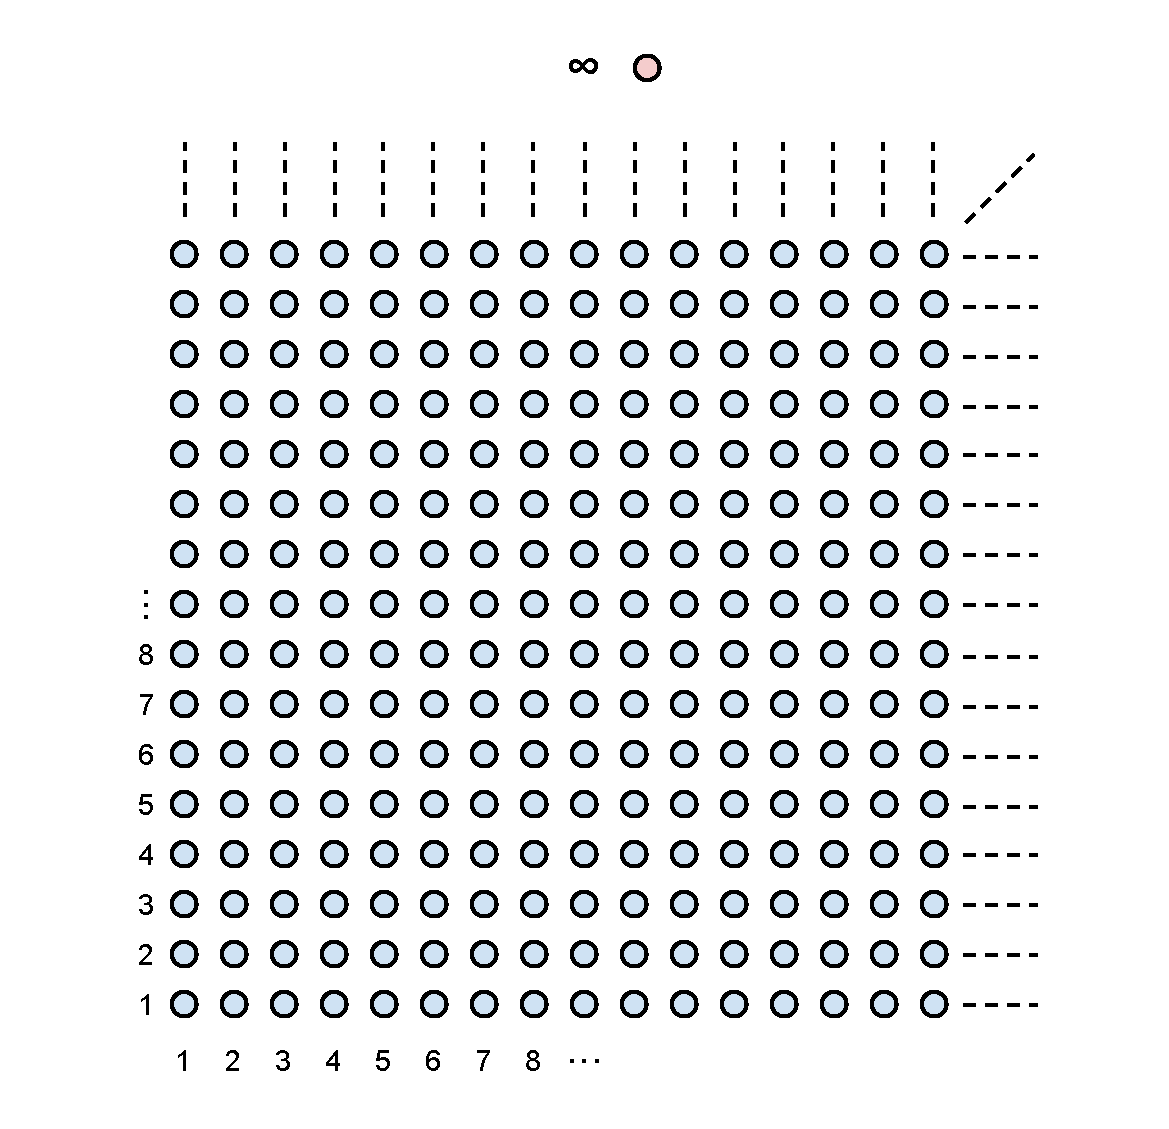
\includegraphics[height=6cm]{images/milky_way}
  \end{center}
\end{frame}
\begin{frame}
  In our so-called Milky Way Space, the dartboards / open sets placed around the point $\infty$ look like this:
  \begin{center}
    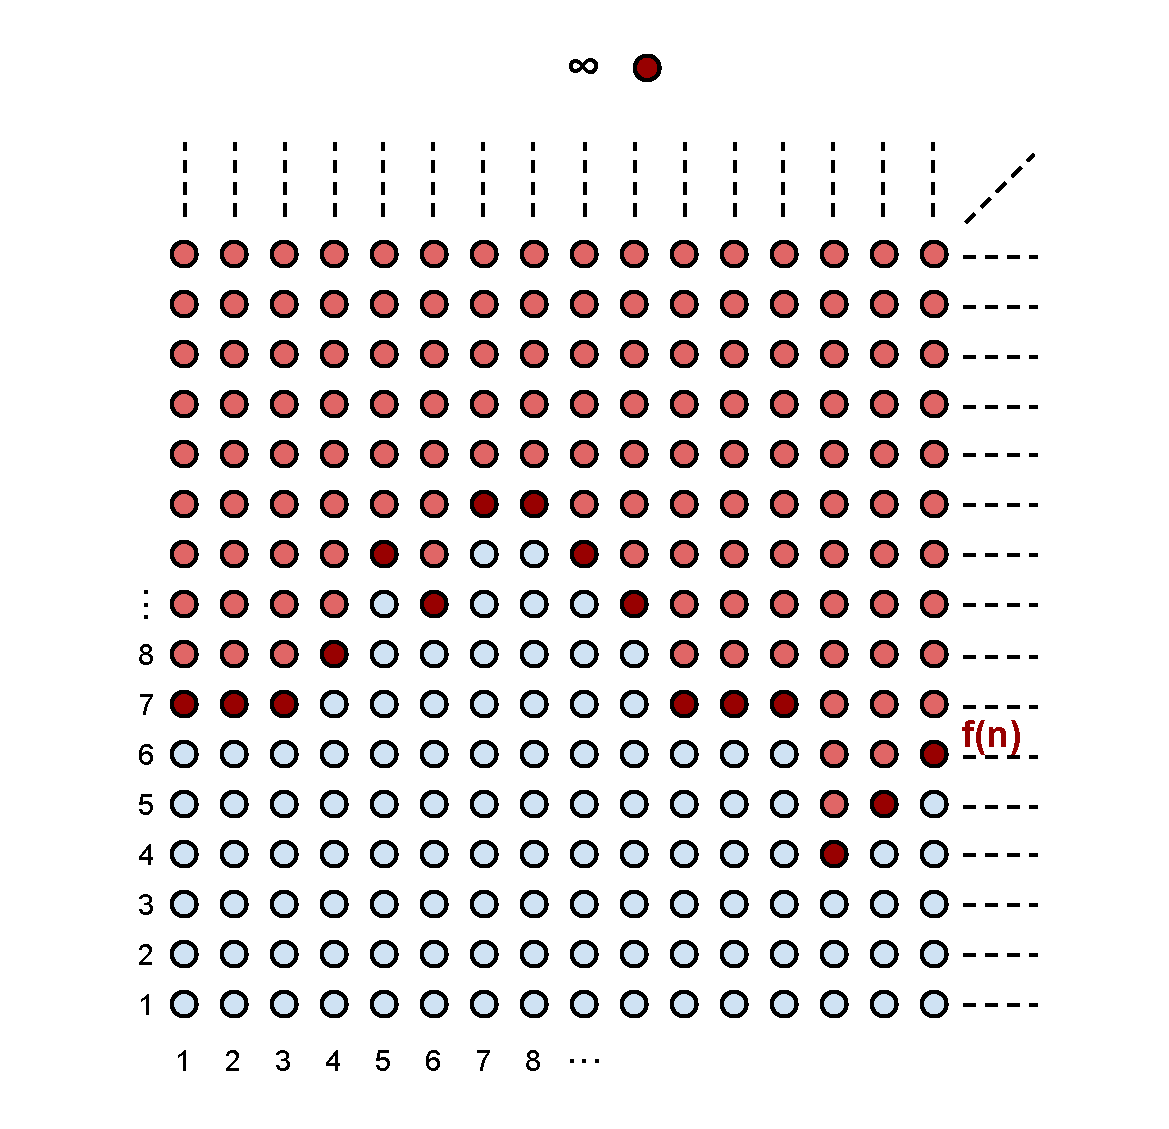
\includegraphics[height=6cm]{images/milky_way_topology}
  \end{center}
\end{frame}

\begin{frame}
  Player P has a \textbf{winning strategy} for Topological Darts when played in the Milky Way Space.
\begin{center}
\begin{tabular}{c|c|c}
Round & Board Picker (O) & Dart Thrower (P) \\\hline
$1$ & $f_1$ & $(1,f_1(1)+1)$ \\
$2$ & $f_2$ & $(2,f_2(2)+1)$ \\
\vdots & \vdots & \vdots \\
$n$ & $f_n$ & $(n,f_n(n)+1)$ \\
\vdots & \vdots & \vdots \\
\end{tabular}
\end{center}
  The dartboard given by $g(n)=f_n(n)+3$ misses all points played by P.
\end{frame}
\begin{frame}
Round 1
\begin{center}
    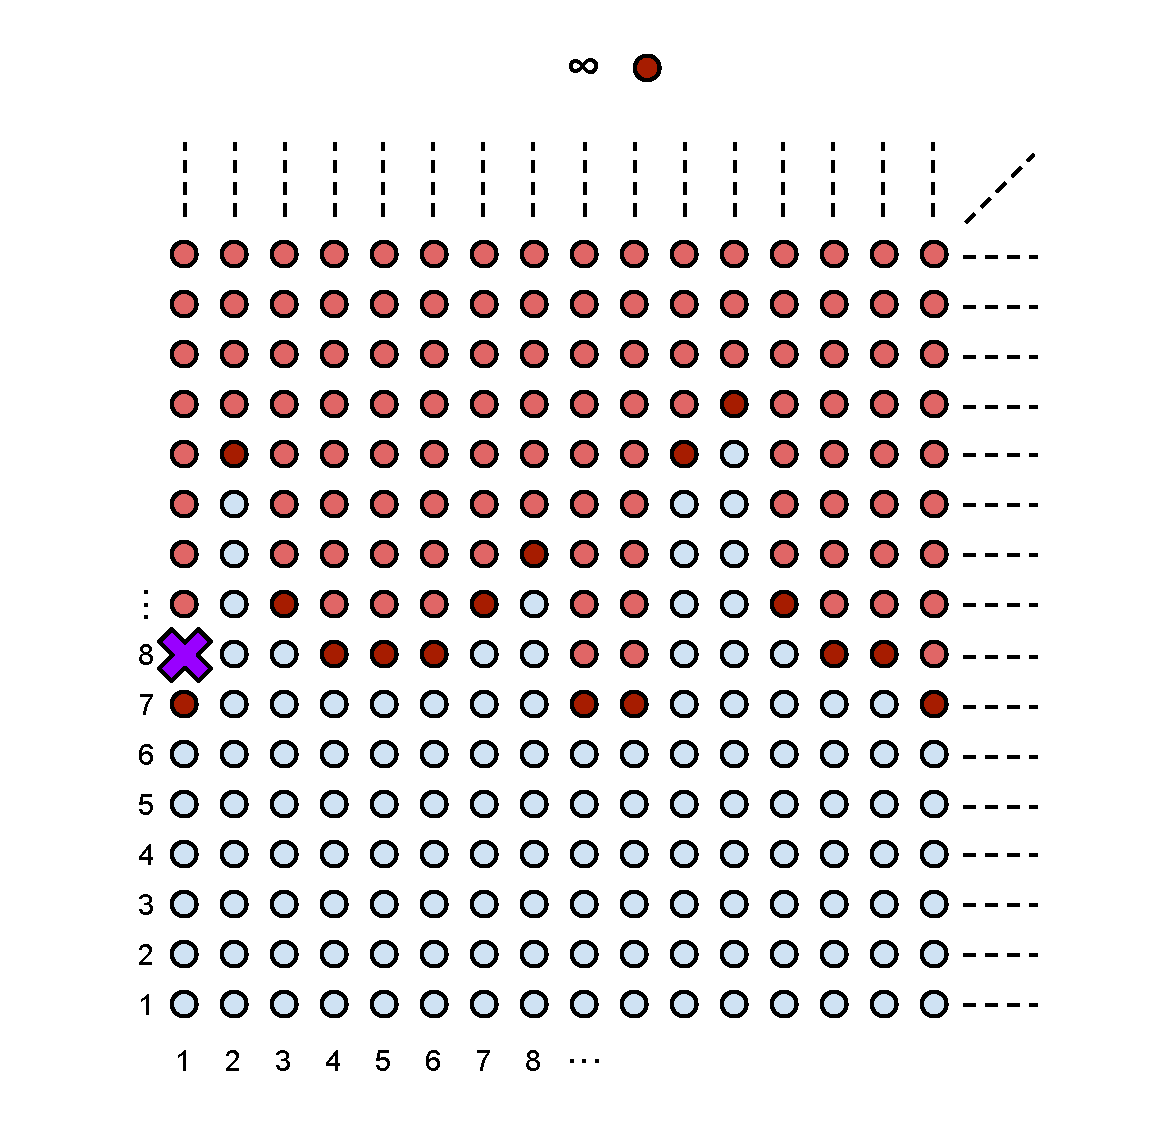
\includegraphics[height=7cm]{images/topdarts_fan_p1}
  \end{center}
\end{frame}
\begin{frame}
Round 2
\begin{center}
    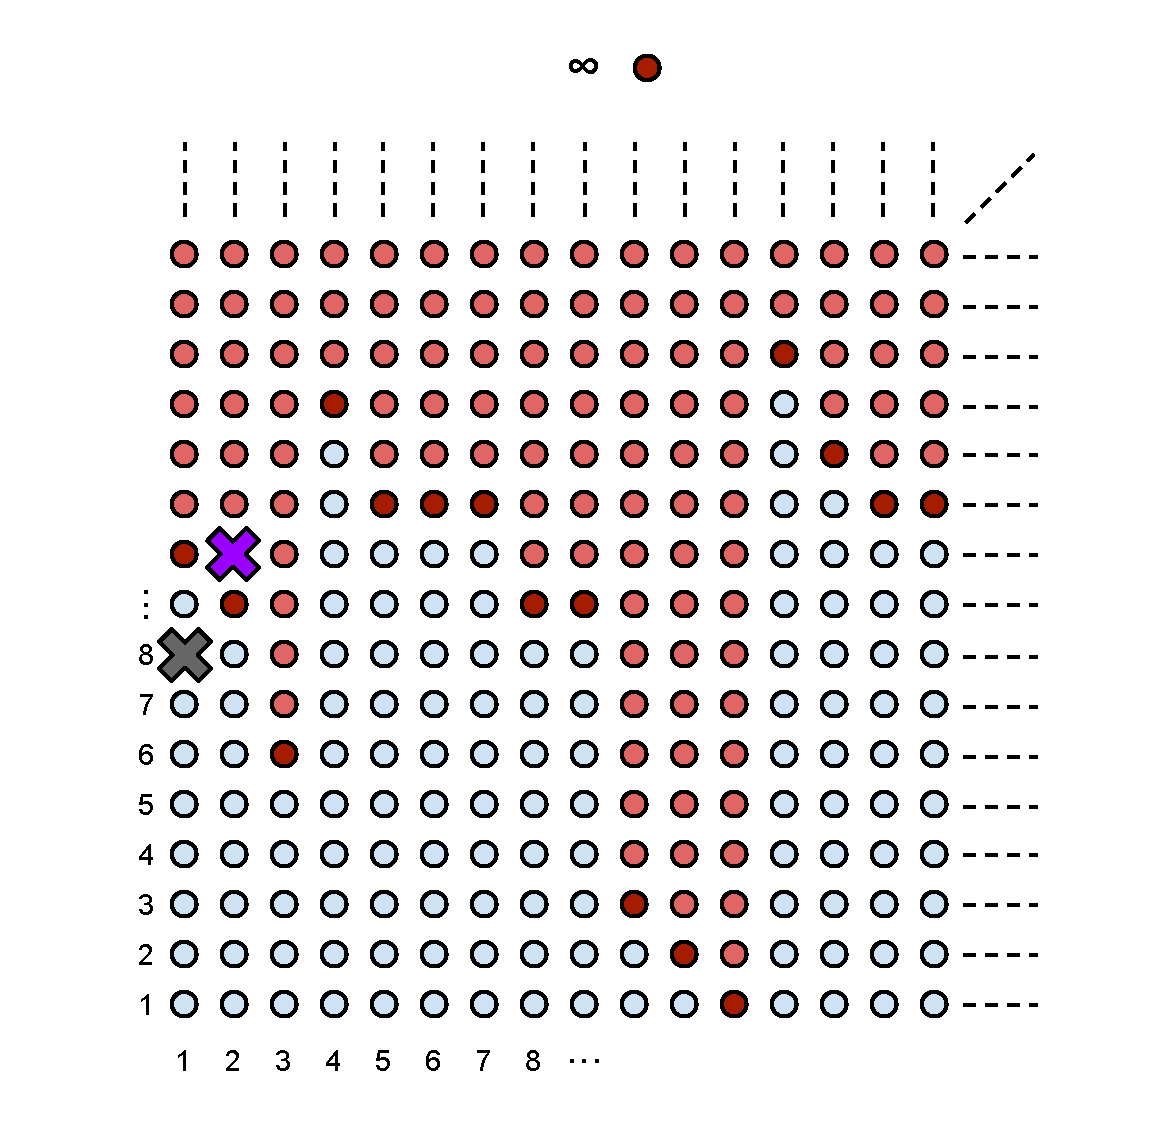
\includegraphics[height=7cm]{images/topdarts_fan_p2}
  \end{center}
\end{frame}
\begin{frame}
Round 3
\begin{center}
    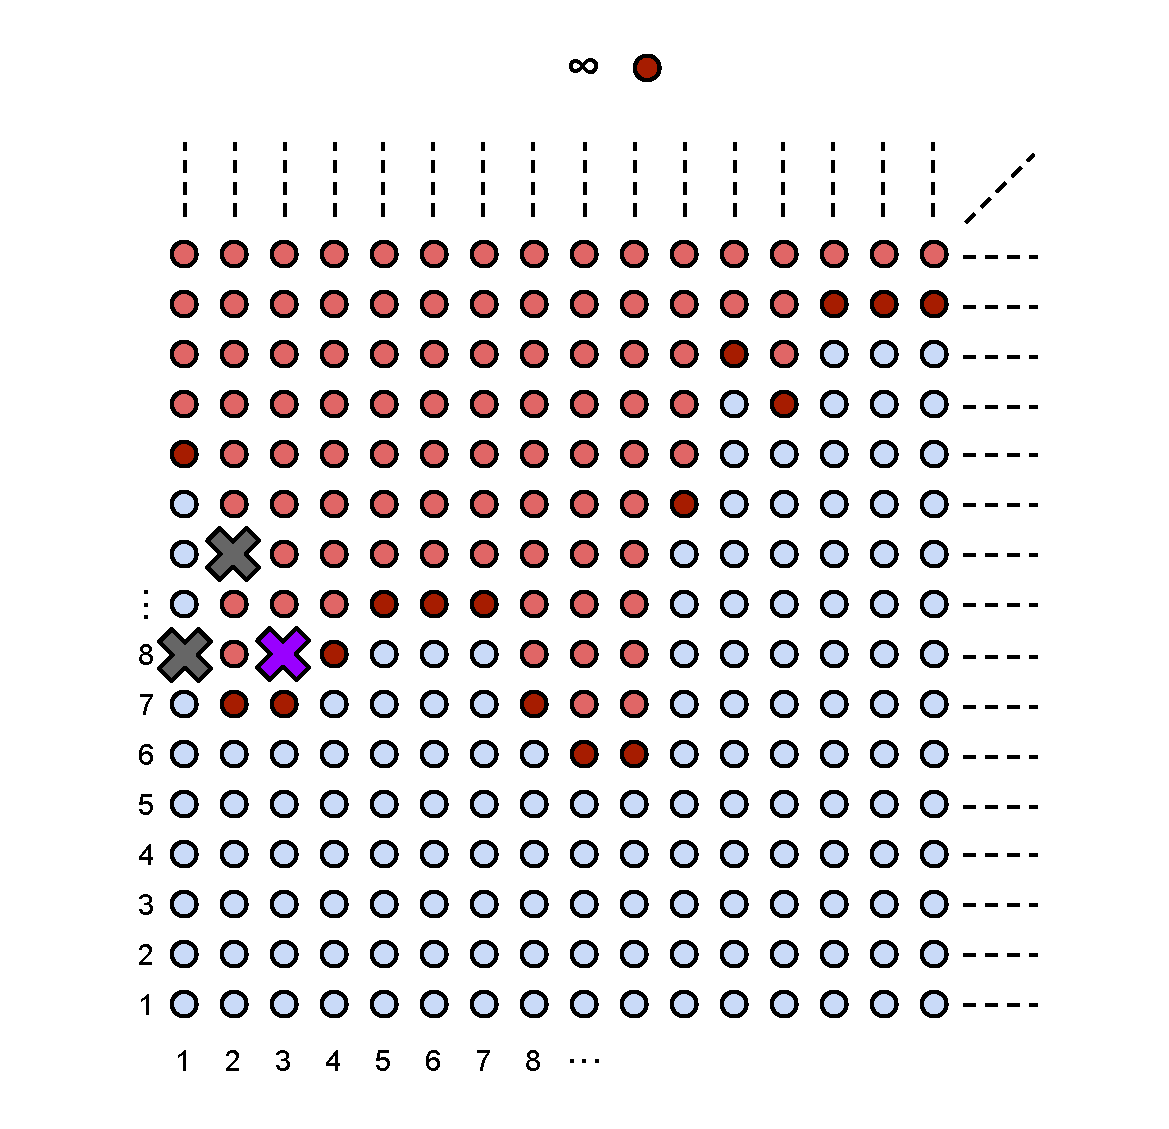
\includegraphics[height=7cm]{images/topdarts_fan_p3}
  \end{center}
\end{frame}
\begin{frame}
After the game...
\begin{center}
    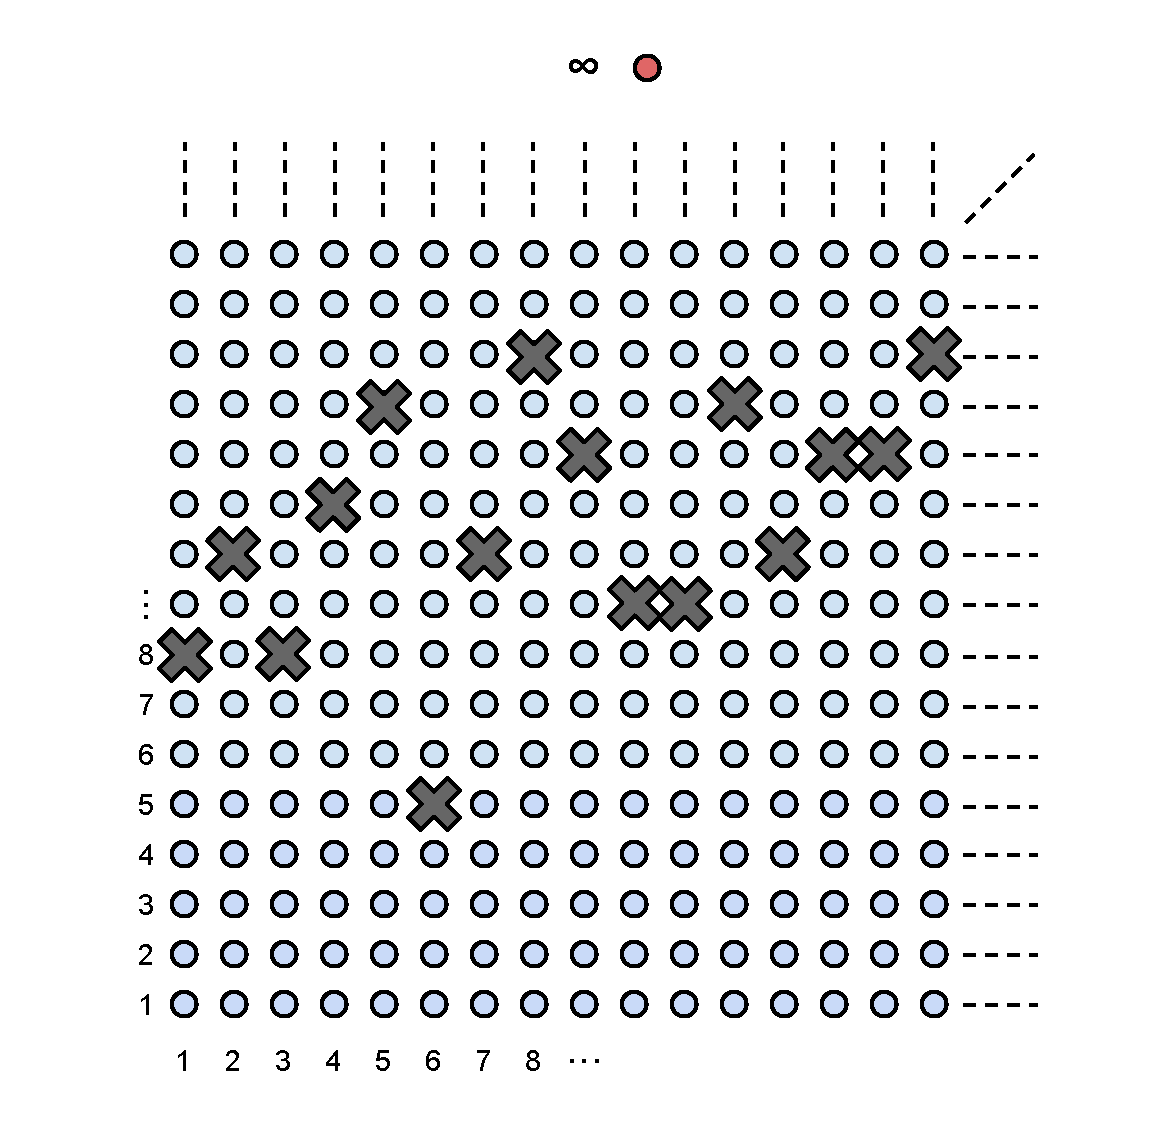
\includegraphics[height=7cm]{images/topdarts_fan_finale}
  \end{center}
\end{frame}
\begin{frame}
After the game...
\begin{center}
    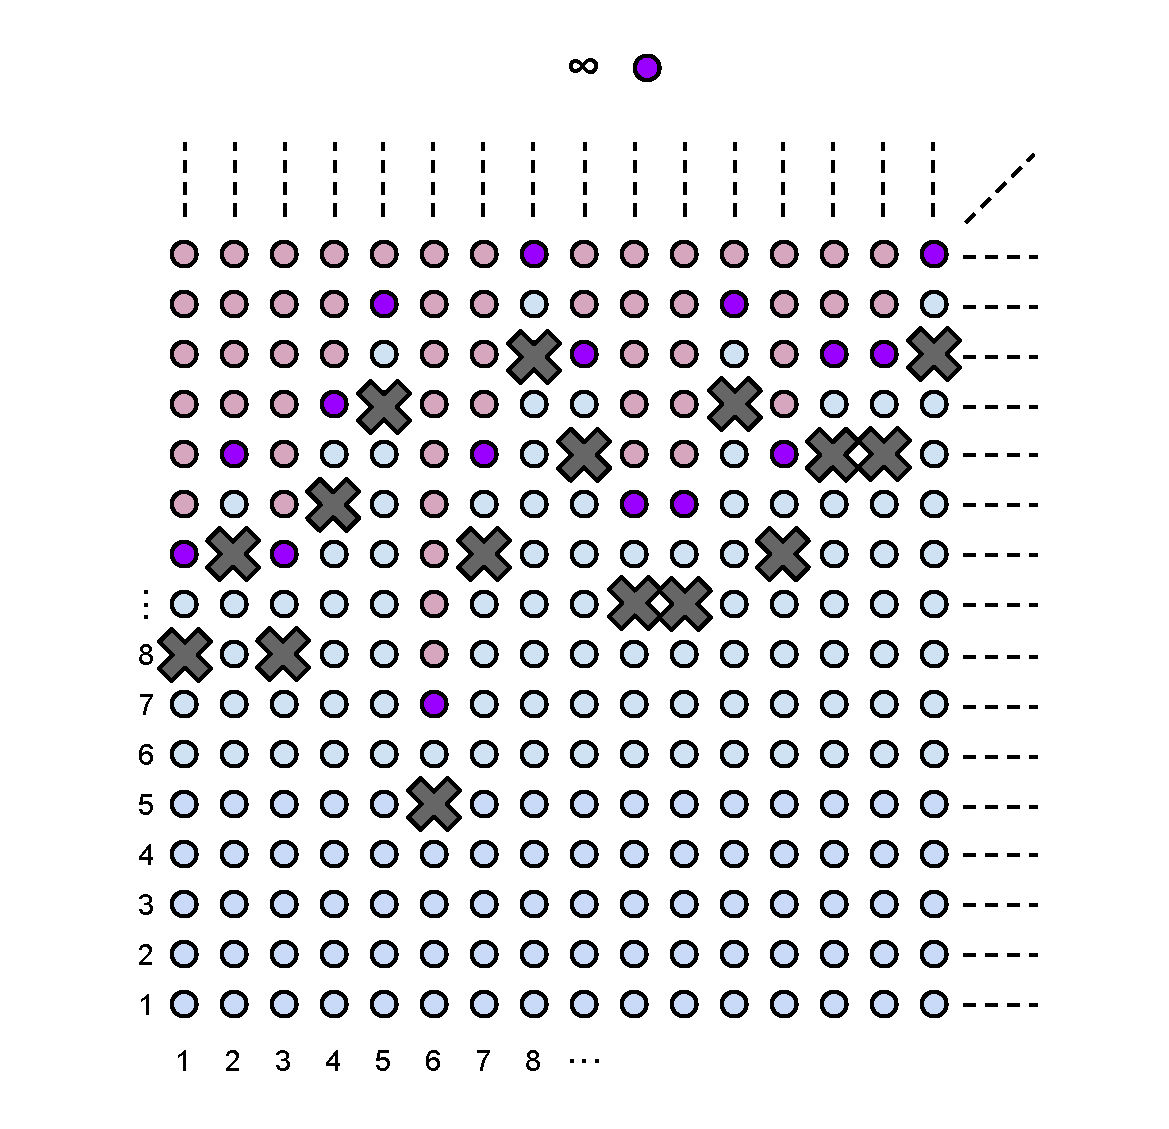
\includegraphics[height=7cm]{images/topdarts_fan_finale2}
  \end{center}
\end{frame}


\subsection{So what?}

\begin{frame}{So what?}
  \begin{itemize}
    \item
      We care about these games because they provide very slick ways of describing possible structures of a topological space.
    \pause
      \begin{itemize}
        \item
          A topological space $X$ is an ``$\alpha_2$ Fr\'echet-Urysohn'' space if for each subset $A$ of $X$, and each point $x \in \overline{A}$, there exists a sequence of points in $A$ converging to $x$, and for each countable collection of sequences coverging to $x$, there is yet another sequence converging to $x$ which intersects each of these infinitely many times.
      \end{itemize}
  \end{itemize}
\end{frame}

\begin{frame}
  \begin{itemize}
    \item
      It's much simpler to say this:
    \pause
      \begin{itemize}
        \item
          A topological space $X$ is an ``$\alpha_2$ Fr\'echet-Urysohn'' space if and only if Player P cannot find a winning strategy in a game of Topological Darts played in $X$.
      \end{itemize}
    \pause
    \item
      So we know the $xy$-plane is ``$\alpha_2$ Fr\'echet-Urysohn'' (we found a winning strategy for Player O, so Player P doesn't have one), but the Milky Way Space isn't (we found a winning strategy for Player P).
  \end{itemize}
\end{frame}

\section{Limited Information Games}

\subsection{What are these?}

\begin{frame}{Consquences of Limited Information}
  \begin{itemize}
    \item
      So far we've assumed both players have perfect memories. But what happens if a player can only remember (for example) the most recent move of her opponent?
    \pause
    \item
      My reseach is concerned with the consquences of one player having this sort of ``limited information'' in a topological game.
  \end{itemize}
\end{frame}
\begin{frame}
  In the $xy$-plane, Player O has a \textbf{tactical} strategy for Topological Darts which relies on only the most recent move of her opponent:
  \begin{itemize}
    \item
      During round (?), Player O sees that Player P has just thrown a dart at $(x_?,y_?)$.
    \item
      Although Player O doesn't know anything else about what's happened during the game, she places a dartboard with center $(0,0)$ and radius $\frac{\sqrt{x_?^2+y_?^2}}{2}$.
  \end{itemize}
\end{frame}
\begin{frame}
Here's how it plays out:
\begin{center}
\begin{tabular}{c|c|c|c}
 & Player O & Player P & Dist. from $(0,0)$ \\\hline
$1$ & $x^2+y^2 < 1$ & $(x_1,y_1)$ & $< 1$ \\
$2$ & $x^2+y^2 < \frac{x_1^2+y_1^2}{4}$ & $(x_2,y_2)$ & $< \frac{\sqrt{x_1^2+y_1^2}}{2} < \frac{1}{2}$ \\
$3$ & $x^2+y^2 < \frac{x_2^2+y_2^2}{4}$ & $(x_3,y_3)$ & $< \frac{\sqrt{x_2^2+y_2^2}}{2} < \frac{1}{2}\frac{1}{2}=\frac{1}{4}$ \\
\vdots & \vdots & \vdots & \vdots \\
$n$ & $x^2+y^2 < \frac{x_{n-1}^2+y_{n-1}^2}{4}$ & $(x_n,y_n)$ & $< \frac{\sqrt{x_{n-1}^2+y_{n-1}^2}}{2} < \frac{1}{2}\frac{1}{2^{n-1}} = \frac{1}{2^n}$ \\
\vdots & \vdots & \vdots & \vdots \\
\end{tabular}
\end{center}
\end{frame}
\begin{frame}
  But in the Milky Way Space, Player P does \textit{not} have a winning tactical strategy, \pause\textit{even though she has a unbeatable perfect information strategy}.
\end{frame}
\begin{frame}
Round ?
\begin{center}
    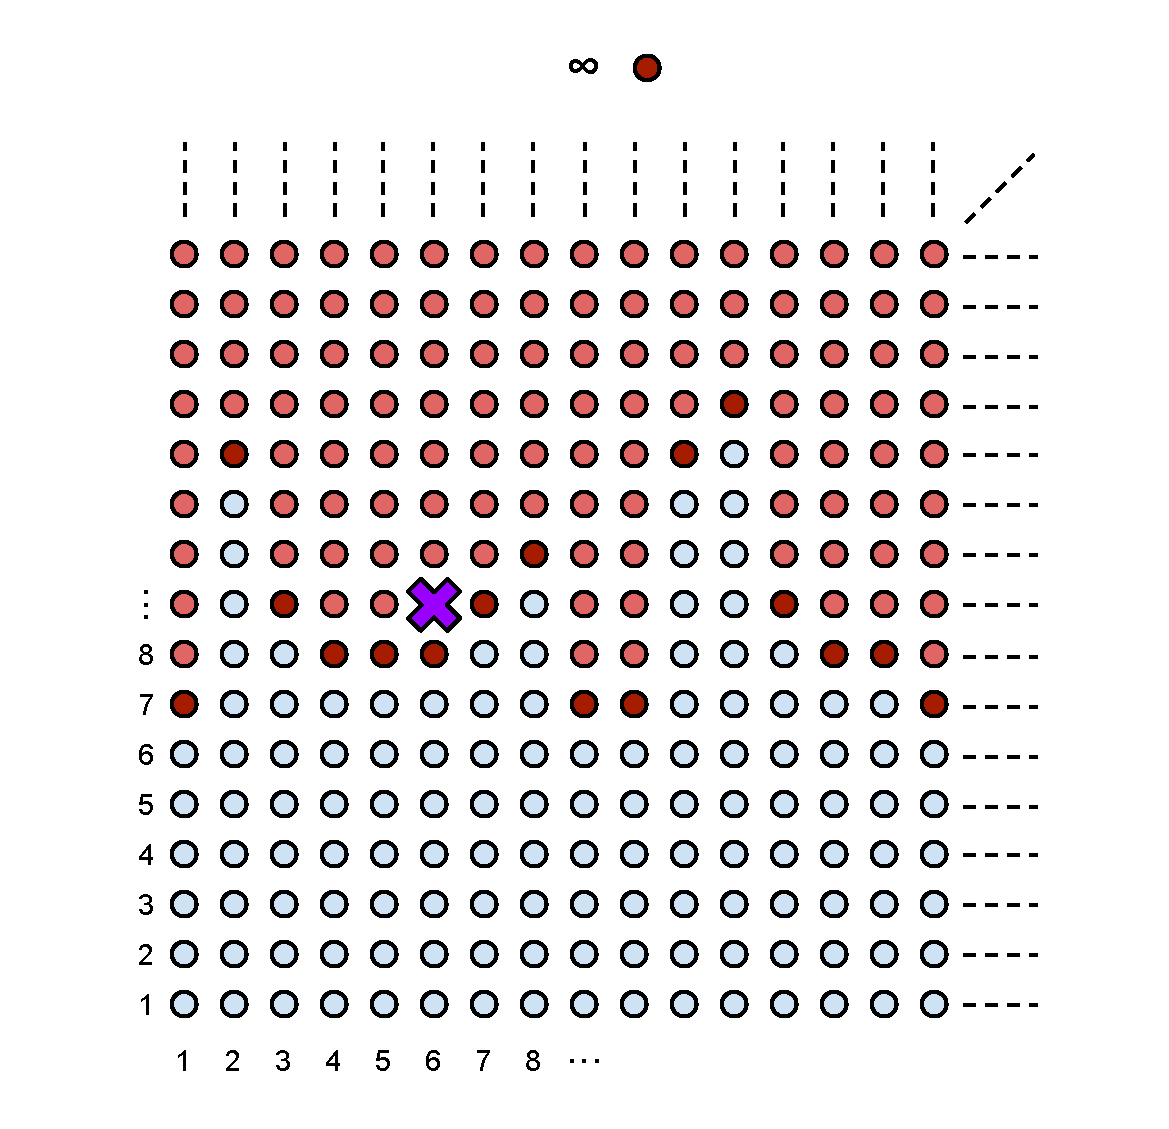
\includegraphics[height=7cm]{images/topdarts_fan_p1_tactic}
  \end{center}
\end{frame}
\begin{frame}
Round ?!
\begin{center}
    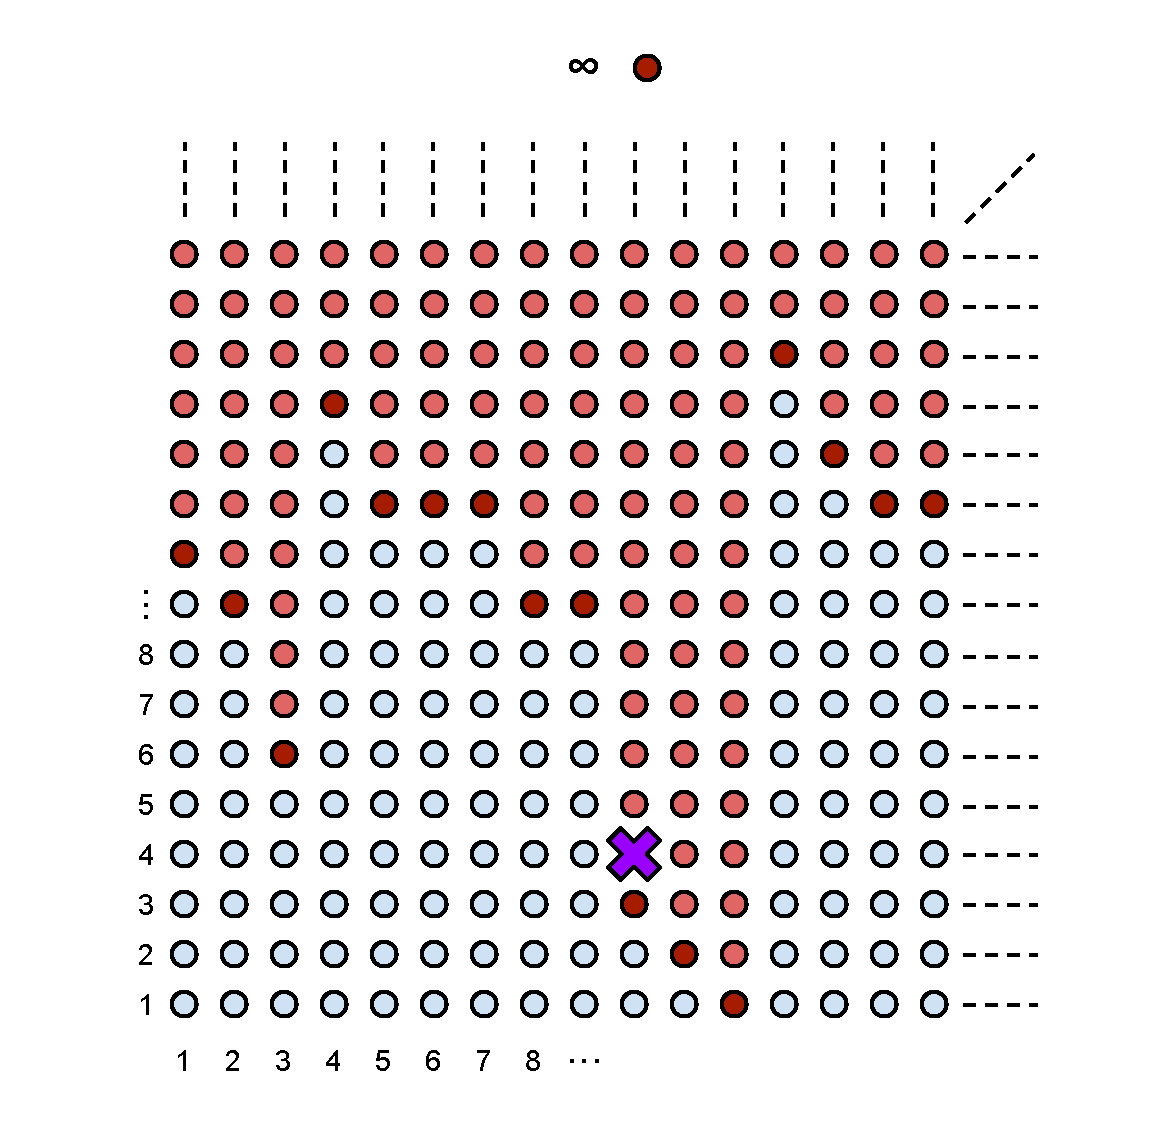
\includegraphics[height=7cm]{images/topdarts_fan_p2_tactic}
  \end{center}
\end{frame}
\begin{frame}
Round ?\#!?@
\begin{center}
    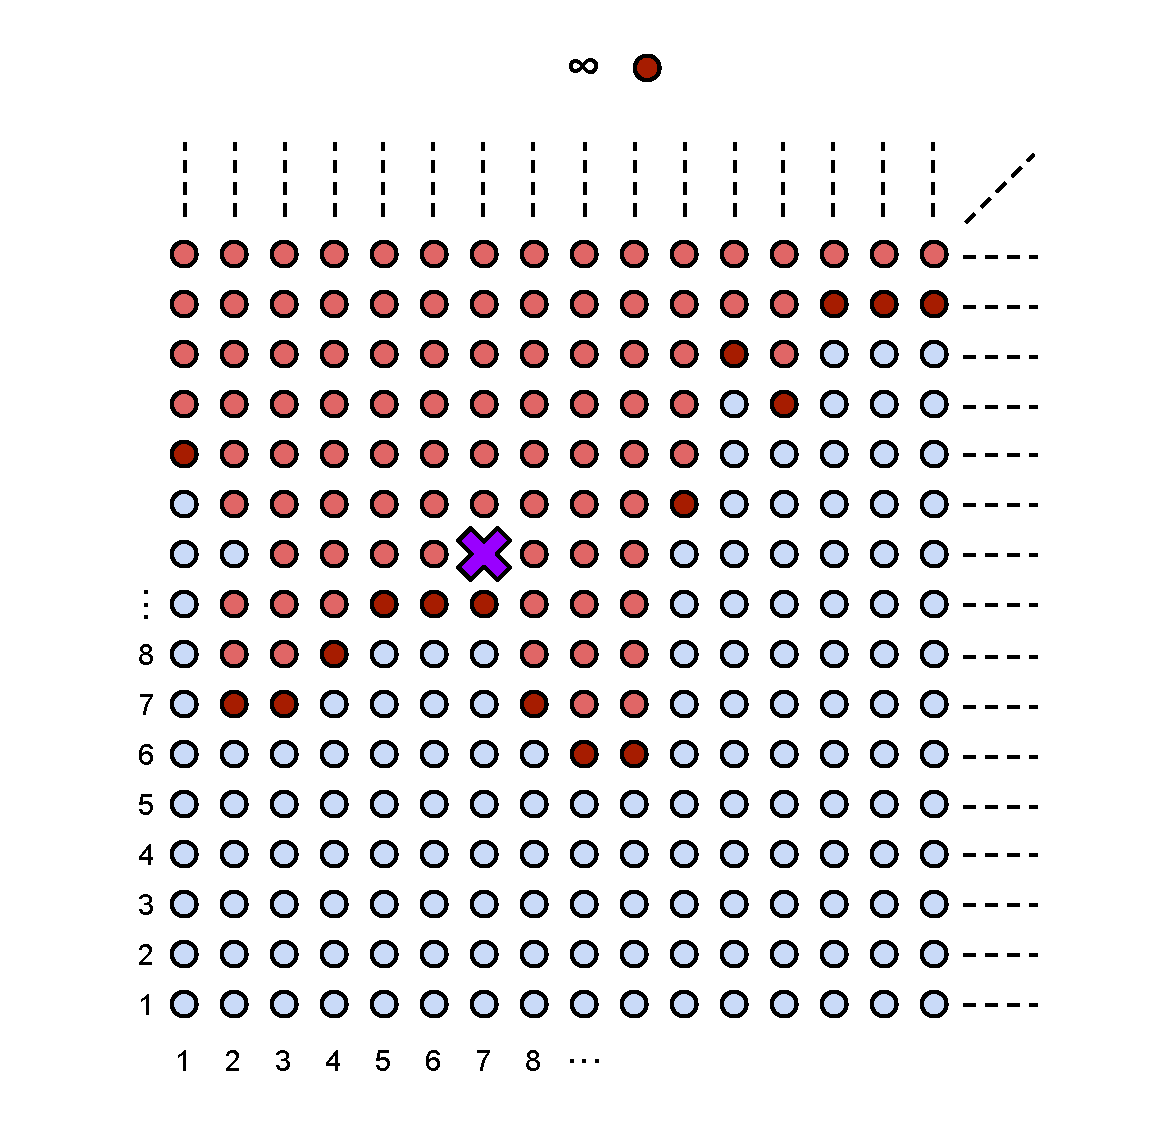
\includegraphics[height=7cm]{images/topdarts_fan_p3_tactic}
  \end{center}
\end{frame}
\begin{frame}
After the game...
\begin{center}
    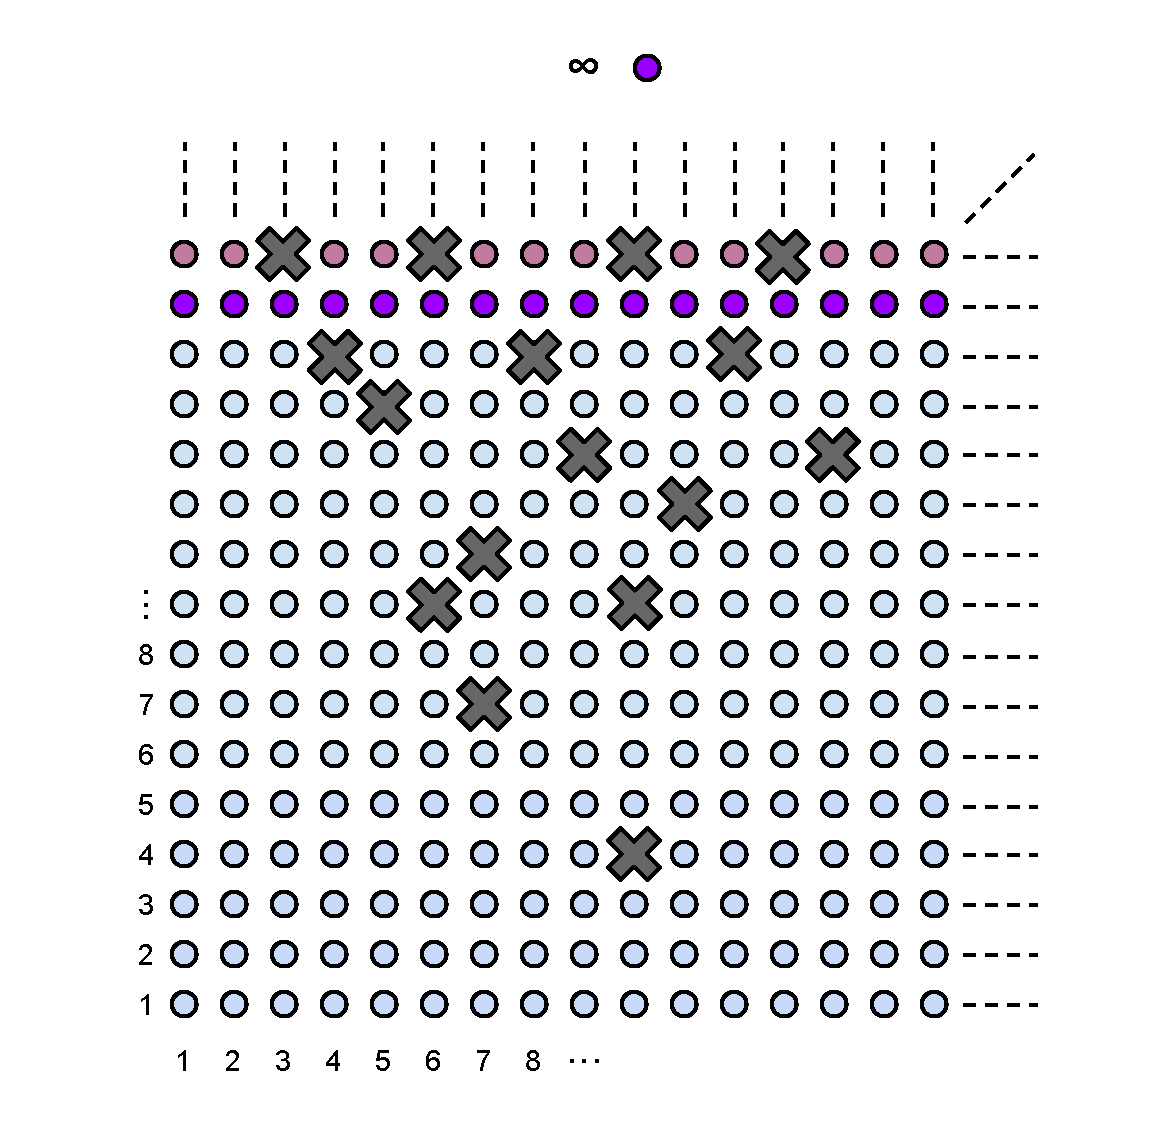
\includegraphics[height=7cm]{images/topdarts_fan_finale_tactic}
  \end{center}
\end{frame}

\begin{frame}
  \begin{itemize}
    \item
      The presence or absence of perfect information strategies in a topological game characterize some structure of the space played upon - same goes for limited information strategies.

      {\tiny Assume all spaces are countably-tight, locally-compact. $\oneptcomp{X}$ is the one-point compactification of $X$.}
    \pause
    \begin{itemize}
      \item
        A topological space $X$ is \textbf{metaLindel\"of} if and only if Player O has a winning strategy for Topological Darts played in $\oneptcomp{X}$.
      \pause
      \item
        A topological space $X$ is \textbf{metacompact} if and only if Player O has a winning \textbf{tactical} strategy for Topological Darts played in $\oneptcomp{X}$.
    \end{itemize}
  \end{itemize}
\end{frame}

\subsection{My Results}

\begin{frame}{So what have you done?}
My main questions: \pause
  \begin{itemize}
    \item ``How can we strengthen existing results from the literature concerning topological games?''
    \pause
    \item ``What common topological properties are characterized by the existance or absence of limited information strategies?''
  \end{itemize}
\pause
Here are some examples of my results:
\end{frame}

\begin{frame}
  Gary Gruenhage (Auburn) has shown that, for locally compact spaces,
    \[
      X \text{ is metacompact} \Leftrightarrow O \tactwin \congame{\oneptcomp{X}}{\infty}
    \]
  {\tiny $\congame{X}{x}$ is Topological Darts.}
  \pause
  \begin{itemize}
    \item
      I have shown further that 
    \[
      X \text{ is metacompact} \Leftrightarrow O \tactwin \clusgame{\oneptcomp{X}}{\infty}
    \]
    \pause
    \item
      I've also proven there exists a space which suggests the following conjecture:
    \[
      X \text{ is metacompact} \Leftrightarrow O \ktactwin{k} \congame{\oneptcomp{X}}{\infty} \, ?
    \]
  \end{itemize}
\end{frame}

\begin{frame}
  Peter J. Niykos (S. Carolina) has shown that 
    \[
      O \not\markwin \congame{\oneptcomp{\omega_1}}{\infty}
    \]
  {\tiny A Mark\"ov strategy depends on the most recent move of the opponent and the round number.}
  \pause
  \begin{itemize}
    \item
      I've improved this to show that for any $\kappa \geq \omega_1$ and positive integer $k$, $O \not\kmarkwin{k} \congame{\oneptcomp{\kappa}}{\infty}$
    \pause
    \item
      I've also shown that while $O \not\kmarkwin{k} \clusgame{\oneptcomp{\kappa}}{\infty}$ for $\kappa>\omega_1$, $O \markwin \clusgame{\oneptcomp{\omega_1}}{\infty}$
  \end{itemize}
\end{frame}

\begin{frame}
  I've also introduced a new type of limited information strategy: \textbf{predetermined} strategies which ignore the moves of the opponent and only use the round number.
  \pause
  \begin{itemize}
    \item
    For locally compact spaces:
      \[
        X \text{ is Lindel\"of} \Leftrightarrow X \text{ is } \sigma\text{-compact} \Leftrightarrow X \text{ is hemicompact}
      \]
      \[
        \Leftrightarrow K \prewin \lfkpgame{X} \Leftrightarrow K \prewin \lfklgame{X}
      \]
    \pause
    \item
    For Hausdorff $k$-spaces:
      \[
        X \text{ is } k_\omega \Leftrightarrow X \text{ is hemicompact}
      \]
      \[
        \Leftrightarrow K \prewin \lfkpgame{X} \Leftrightarrow K \prewin \lfklgame{X}
      \]
  \end{itemize}
\end{frame}

\section{Thanks / Questions?}

\begin{frame}{Thank you!}
  \begin{itemize}
    \item Thanks goes to my advisor Gary Gruenhage, and regular attendees of the set-theoretic topology seminar for their feedback and support.
    \item A BIG thank-you goes to the Graduate Student Council for organizing the Graduate Scholars' Forum and assisting with AU Research Week.
    \item And most of all, thanks to the volunteer judges for taking time out of their busy schedules to support graduate student research at Auburn!
  \end{itemize}
Any questions?

{\tiny Full presentation available on: <http://www.stevenclontz.com/AURW2013/>}
\end{frame}
\begin{frame}\end{frame}






\begin{frame}{Example of a nontopological infinite game}
  Postscript: Here's a simple example of a nontopological infinite-length game.
  \begin{itemize}
  \item 
    Example game: Player I and Player II take turns picking positive integers $2$ - $9$. A player wins as soon as if the product of all chosen numbers equals a multiple of $18$. If the game never ends, Player I wins as long as she chose $9$ at least once during the game; otherwise Player II wins.
  \end{itemize}
\end{frame}

\begin{frame}
  \begin{itemize}
  \item
    While it's easy to imagine this game never ending (both players always picking $5$ would do it), we can say that Player II has a \textbf{winning strategy}:
    \pause
    \begin{itemize}
      \item Player I can't play any number besides $5$ or $7$ unless it results in a multiple of $18$ - otherwise Player II can make the multiple of $18$ on the next turn.
      \pause
      \item If Player II always plays $7$ in response to $5$ or $7$ being played by Player I, then Player I can never make a multiple of $18$ on her own.
    \end{itemize}
  \pause
  \item 
    Thus one winning strategy for Player II is to always respond with $7$ if Player I chooses $5$ or $7$, and to pick an appopriate number to make a multiple of $18$ otherwise.
  \pause
    \begin{itemize}
      \item 
        The result of any game where Player II sticks to this strategy either involves Player II making a multiple of $18$, or Player I never choosing $9$!
    \end{itemize}
  \end{itemize}
\end{frame}

\end{document}


